\documentclass[usenames,dvipsnames]{beamer}
\usepackage[spanish]{babel}
%\usepackage[latin1]{inputenc}
\usepackage[utf8]{inputenc}
\usepackage{graphicx}
\usepackage{booktabs}

\usepackage{multicol}
\useoutertheme{tree}

% ******************flechas
\usepackage{times}
\usepackage{tikz}
\usepackage{amsmath}
\usepackage{verbatim}
\usetikzlibrary{arrows,shapes}

%********************


% %nro de pagina
% \usepackage{fancyhdr}
% \fancypagestyle{plain}{% en los inicios de capitulo
% % 	\fancyhead{} % get rid of headers
% % 	\renewcommand{\headrulewidth}{0pt} % and the line
% 	\fancyfoot[C]{\thepage} % add page number
% }
%\usepackage{color}
%\usepackage[usenames,dvipsnames,svgnames,table]{xcolor}

%\usetheme{Dresden}
\usetheme[titleformat=smallcaps, numbering=fraction, block=fill]{metropolis}
%\setcounter{tocdepth}{1}
%\usecolortheme{dolphin}
% \useoutertheme{shadow}
% \useinnertheme{rectangles}

% *************************** Caratula


\title[Instituto Sabato]{Diseño y caracterización de esponjas pseudoelásticas}
%\subtitle{}
\author{Prado, Lucia H.}
 \institute{Instituto Sabato 
            \and División Física de Metales - Centro Atómico Bariloche  }
 \date{26/07/2017}




% ************************* Para poner indice antes de cada seccion con dos columnas
 
 
% \AtBeginSection{
% \begin{frame}
%   \frametitle{Índice}
% %   \begin{multicols}{1}
%   \tableofcontents[currentsection]
% %   \end{multicols}
% \end{frame}
% }
% 
% \AtBeginSubsection{
% \begin{frame}
% %   \frametitle{Índice}
%   \begin{multicols}{1}
%   \tableofcontents[currentsection,currentsubsection]
% %   \end{multicols}
% \end{frame}
% }
 %****************************8 Con dos columnas

 %   \AtBeginSection{ 
% \begin{frame} 
%   \frametitle{Índice}
%   \tableofcontents[currentsection]
% \end{frame}
% }
% 
% \AtBeginSubsection{ 
% \begin{frame}
%   \frametitle{Índice}
%   \tableofcontents[currentsection,currentsubsection]
% \end{frame}
% }



% *****************************************8 Diapos 
% \addtocounter{framenumber}{-1}
%\insertframenumber/\inserttotalframenumber
% saca el menu feo
\setbeamertemplate{navigation symbols}{}

 \begin{document}

 %*********************************************************Flechas
 % For every picture that defines or uses external nodes, you'll have to
% apply the 'remember picture' style. To avoid some typing, we'll apply
% the style to all pictures.
\tikzstyle{every picture}+=[remember picture]

% By default all math in TikZ nodes are set in inline mode. Change this to
% displaystyle so that we don't get small fractions.
\everymath{\displaystyle}
%***********************************************************************
 
 
  \frame{\titlepage}
%  
% \begin{frame}
%     \frametitle{Marsupiales}
%     Canguro, Koala, Wombat...
% \end{frame}
% 
% 
% \begin{frame}
%   \frametitle{Marsupiales}
%   \begin{block}{Marsupiales en Australia}
%   Koala, Canguro, Wombat...
%   \end{block}
%       
%   \begin{block}{Marsupiales fuera de Australia}
%   Oposum, Zarigüella...
%   \end{block}
% \end{frame}
% 
% 
% \begin{frame}
%   \frametitle{Animales}
%   \begin{columns}[t]
%     \column{0.5\textwidth}
%     Algunos mamíferos marinos:
%  
%     Ballena, Narval, Cachalote...
% 
%     \column{0.5\textwidth}
%     Y algunos má
%     s:
%  
%     Morsa, León marino, Foca...
%   \end{columns}
% \end{frame}
% 
% 
% \begin{frame}
%   \frametitle{Flores}
%   \begin{itemize}
%   \item<1->{Rosa}
%   \item<2->{Azucena}
%   \item<3->{Margarita}
%   \end{itemize}
% \end{frame}
% 
% 
% \begin{frame}
%   \frametitle{Preguntas}
%   \begin{itemize}
%   \item \alert<1>{¿Cuáles ponen huevos?}
%   \item \alert<3>{¿Cuáles tienen veneno?}
%   \end{itemize}
%      
%   Armadillo, \alert<2,4>{Ornitorrinco}, \alert<2>{Equidna}, Pangolín, Erizo.
% \end{frame}


% ******************
\section{Introducción}


\begin{frame}
\frametitle{Objetivo}

\end{frame}


 \begin{frame}
 \frametitle{Transformación martensítica}

\begin{columns}
 
\column{0.5\textwidth}

\begin{block}{Características}
 \begin{itemize}
  \item En estado sólido
  \item Sin difusión
  \item De primer orden
 \end{itemize}
\end{block}
 
\begin{block}{Formas de transformación}
  \begin{itemize}
  \item \alert<1>{Por temperatura ($M_s$ y $M_f$)}
  \item \alert<2>{Por tensiones (Strain Induced Martensite)}
 \end{itemize}
\end{block}

\column{0.5\textwidth}

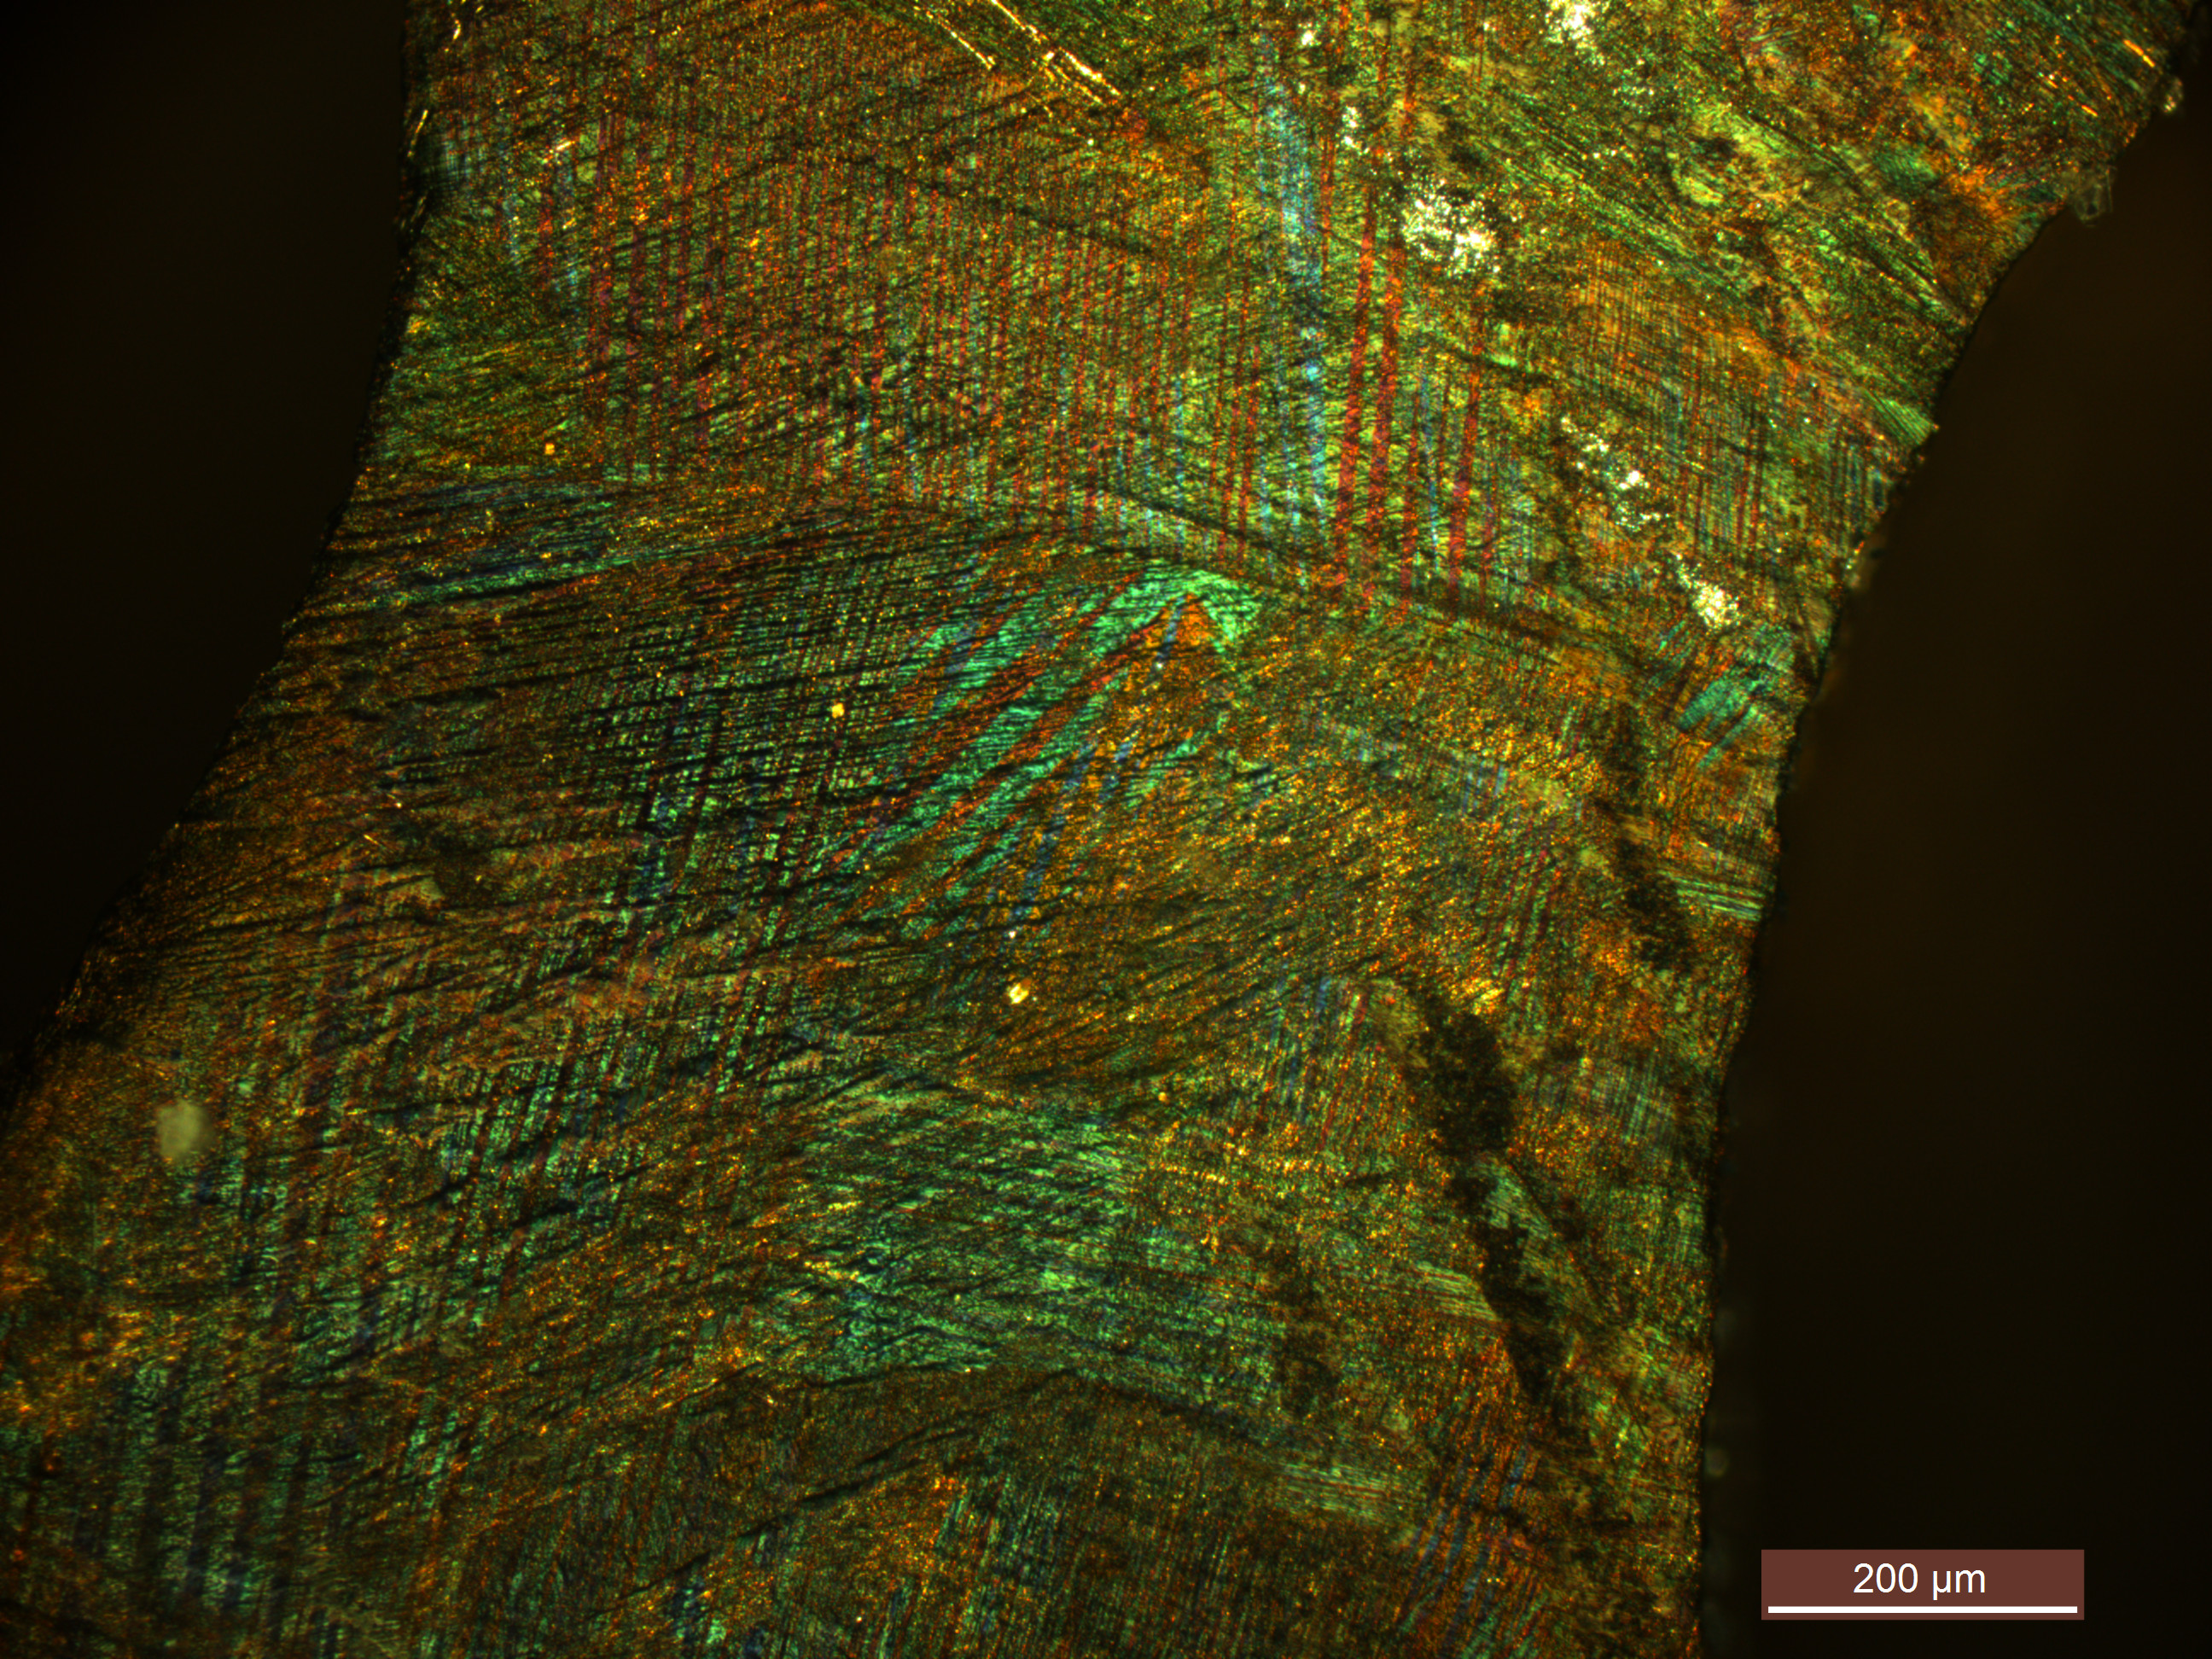
\includegraphics[width=\columnwidth]{img/intro/EspAMicro1.jpg}

\end{columns}
 
\end{frame}

% ******************
% 
% \begin{frame}
% \frametitle{Rigid body dynamics}
% 
% \tikzstyle{na} = [baseline=-.5ex]
% 
% \begin{itemize}[<+-| alert@+>]
%     \item Coriolis acceleration
%         \tikz[na] \node[coordinate] (n1) {};
% \end{itemize}
% 
% % Below we mix an ordinary equation with TikZ nodes. Note that we have to
% % adjust the baseline of the nodes to get proper alignment with the rest of
% % the equation.
% \begin{equation*}
% \vec{a}_p = \vec{a}_o+\frac{{}^bd^2}{dt^2}\vec{r} +
%         \tikz[baseline]{
%             \node[fill=blue!20,anchor=base] (t1)
%             {$ 2\vec{\omega}_{ib}\times\frac{{}^bd}{dt}\vec{r}$};
%         } +
%         \tikz[baseline]{
%             \node[fill=red!20, ellipse,anchor=base] (t2)
%             {$\vec{\alpha}_{ib}\times\vec{r}$};
%         } +
%         \tikz[baseline]{
%             \node[fill=green!20,anchor=base] (t3)
%             {$\vec{\omega}_{ib}\times(\vec{\omega}_{ib}\times\vec{r})$};
%         }
% \end{equation*}
% 
% \begin{itemize}[<+-| alert@+>]
%     \item Transversal acceleration
%         \tikz[na]\node [coordinate] (n2) {};
%     \item Centripetal acceleration
%         \tikz[na]\node [coordinate] (n3) {};
% \end{itemize}
% 
% % Now it's time to draw some edges between the global nodes. Note that we
% % have to apply the 'overlay' style.
% \begin{tikzpicture}[overlay]
%         \path[->]<1-> (n1) edge [bend left] (t1);
%         \path[->]<2-> (n2) edge [bend right] (t2);
%         \path[->]<3-> (n3) edge [out=0, in=-90] (t3);
% \end{tikzpicture}
% \end{frame}
% 

% ********************************************************************

\begin{frame}
\frametitle{Transformación martensítica}

\begin{figure}
\begin{tikzpicture}
\pgftext{%
 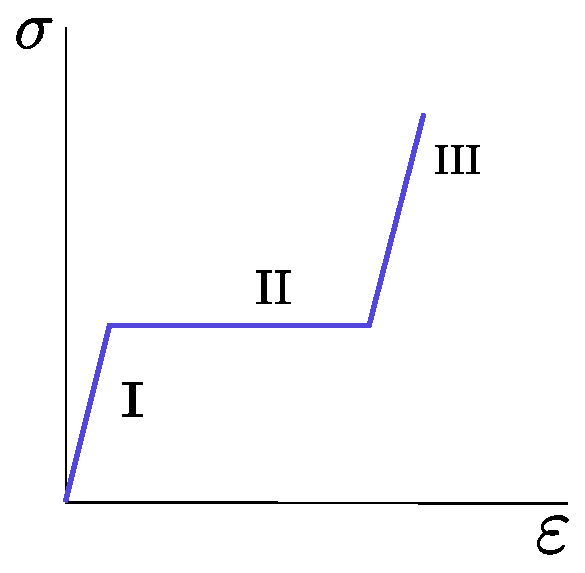
\includegraphics[width=0.4\textwidth]{img/intro/SigmavsDef.eps}
}%

\node (I) at (-1.2,-0.9) {};
\node (II) at (0, 0) {};
\node (III) at (1.5, 1) {};
\node[align=right] (It)   at (5.25, -0.9) {Deformación elástica de $\beta$};
\node[align=right] (IIt)  at (6,0) {Formación y crecimiento de placas};
\node[align=right] (IIIt) at (4.8, 1) {Deformación elástica};
% 
\path[->]<1-> (I) edge [dashed] (It);
\path[->]<1-> (II) edge [dashed] (IIt);
\path[->]<1-> (III) edge [dashed] (IIIt);

\end{tikzpicture}
\end{figure}

 
\end{frame}

%%%%%%%%%%%%%%%%%%%%%%%%%%%%%%%%%%%%%%%%%%%%%%%%%%%%%%%%%%%%%%%%%%%%%%%%%%%%%%%%%%%%%%%%%%%%%5

\begin{frame}
\frametitle{Transformación martensítica}

\begin{columns}
\column{0.6\textwidth}

\begin{block}{Ley de Schmid}
\begin{equation*}
 \tau_{R}= \sigma cos(\lambda)cos(\phi)
\end{equation*}

\begin{center}
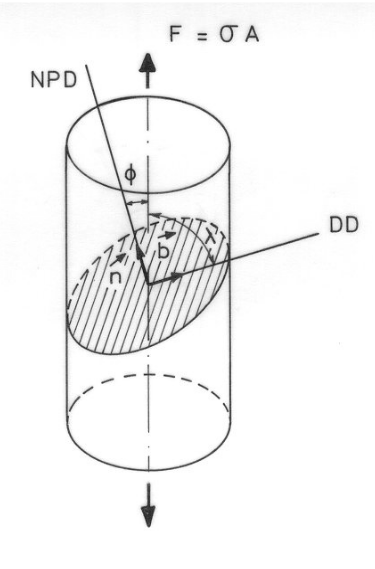
\includegraphics[width=0.5\columnwidth]{img/intro/tension.png}
\end{center}

\end{block}

\column{0.4\textwidth}

\pause
\begin{block}{Monocristal}
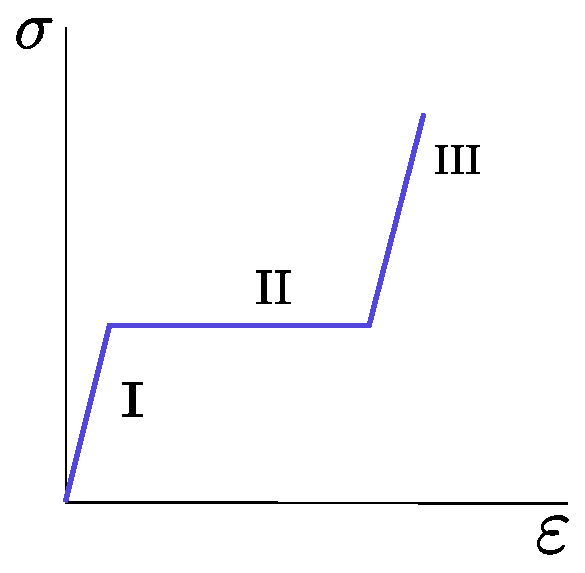
\includegraphics[height=0.35\textheight]{img/intro/SigmavsDef.eps} 
\end{block}

\pause
\begin{block}{Policristal}
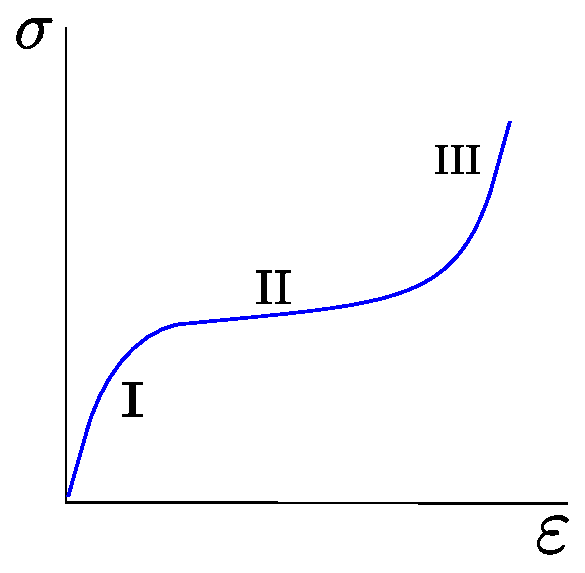
\includegraphics[height=0.35\textheight]{img/intro/SigmavsDefPoli.eps}
\end{block}

\end{columns}

% \end{center}
% \end{multicols}
 
\end{frame}

\begin{frame}
\frametitle{Tensión de transformación}

\begin{columns}
\column{0.4\textwidth}

\begin{block}{Clausius-Clapeyron}
\begin{equation*}
 \frac{d \tau_{R}}{dT}=\frac{\Delta S}{\Delta V} 
\end{equation*}
\end{block}

\begin{itemize}
 \item $\uparrow T \rightarrow \, \uparrow \tau_{R}$
 \item $\tau_{R} = 0  \rightarrow T=M_{s}$
\end{itemize}

\column{.4\textwidth}
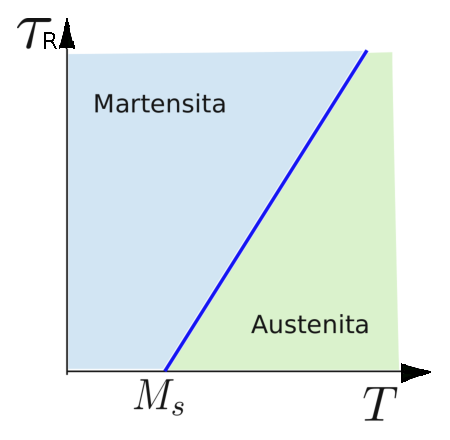
\includegraphics[width=\columnwidth]{img/intro/Clapeyron.eps}

\end{columns}


\end{frame}


\begin{frame}

\frametitle{Pseudoplasticidad}


Fricción por movimiento de interfases y creación de defectos.

\vfill

\begin{columns}
\column{0.4\textwidth}
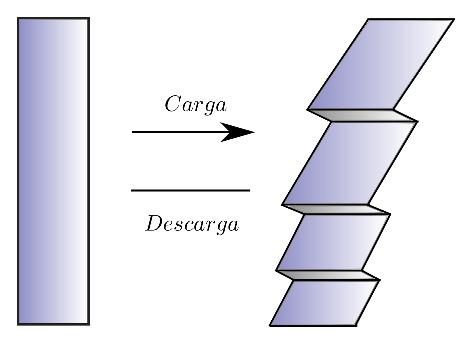
\includegraphics[width=\columnwidth]{img/intro/HisteresisEsquema.eps}
\column{0.4\textwidth}
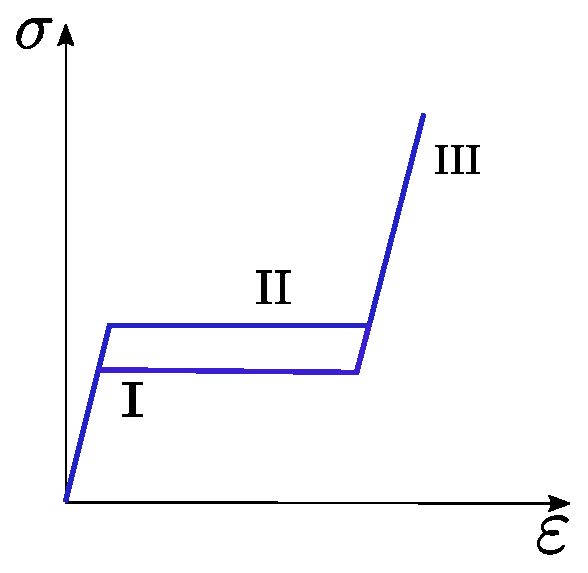
\includegraphics[width=\columnwidth]{img/intro/Histeresis.eps}
 
\end{columns}

\end{frame}

%%%%%%%%%%%%%%%%%%%%%%%%%%%%%%%%%%%%%%%%%%%%%%%%%%%%%%%

%%%%%%%%%%%%%%%%%%%%%%%%%%%%%%%%%%%%%%%%%%%%%%%%%%%%%%


\begin{frame}
\frametitle{Memoria de forma}

 \begin{itemize}
  \item Forma inicial en estado austenítico
  \item Enfriamiento a $T<M_{s}$
  \item Deformación en estado martensítico
  \item Calentamiento a $T>A_{f}$
 \end{itemize}


\begin{center}
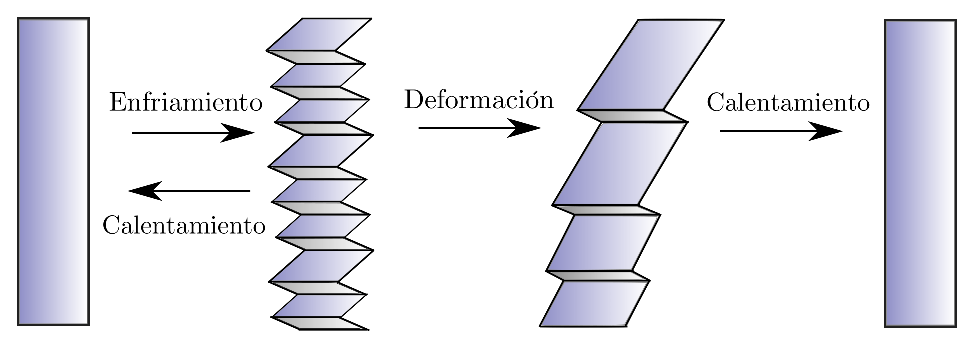
\includegraphics[width=0.9\textwidth]{img/intro/Trans.eps} 
% 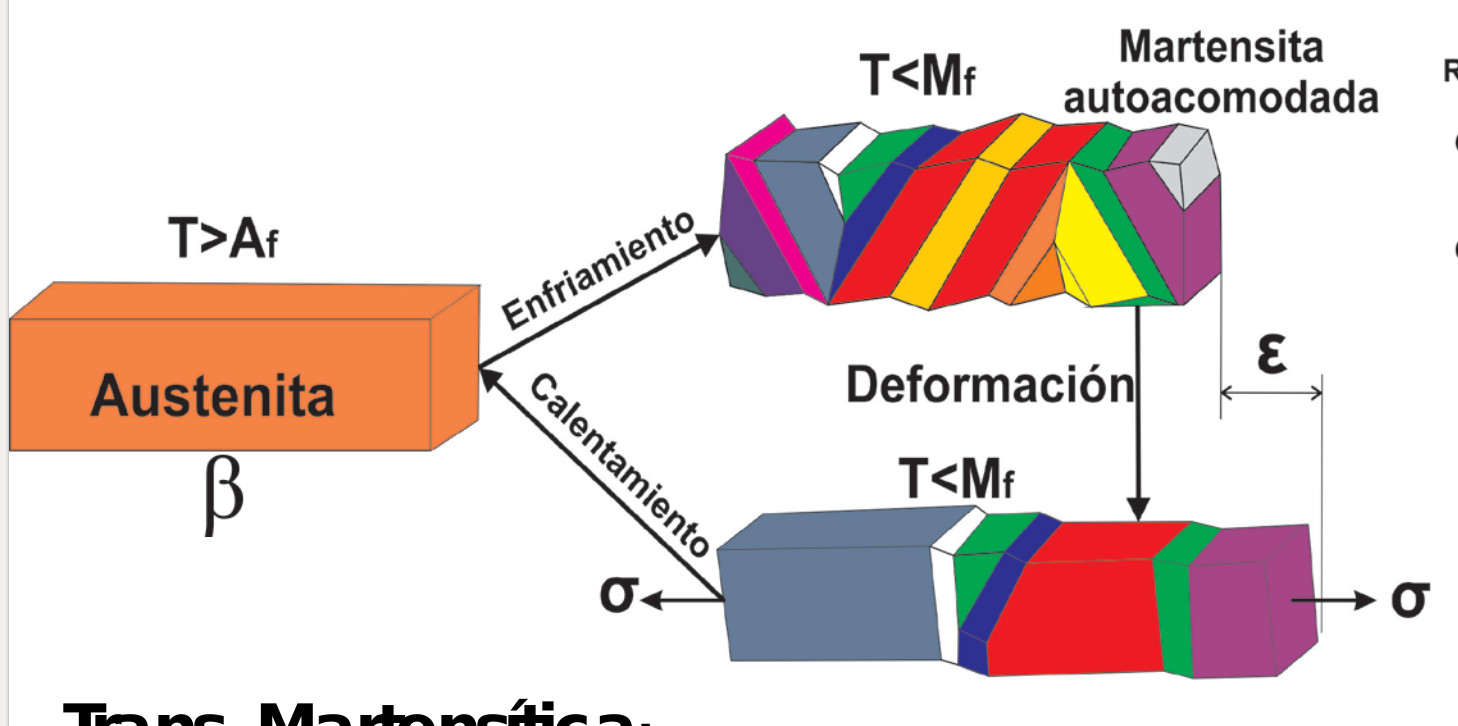
\includegraphics[width=0.8\textwidth]{img/intro/memoria.jpg}
\end{center}

% Cosas que juegan en contra:
% \begin{itemize}
%   \item Envejecimiento y estabilización
%   \item Anclaje entre placas de martensita
%  \end{itemize}

\end{frame}

%*************************

% ************************ 

\begin{frame}
\frametitle{Aleación Cu-Zn-Al}
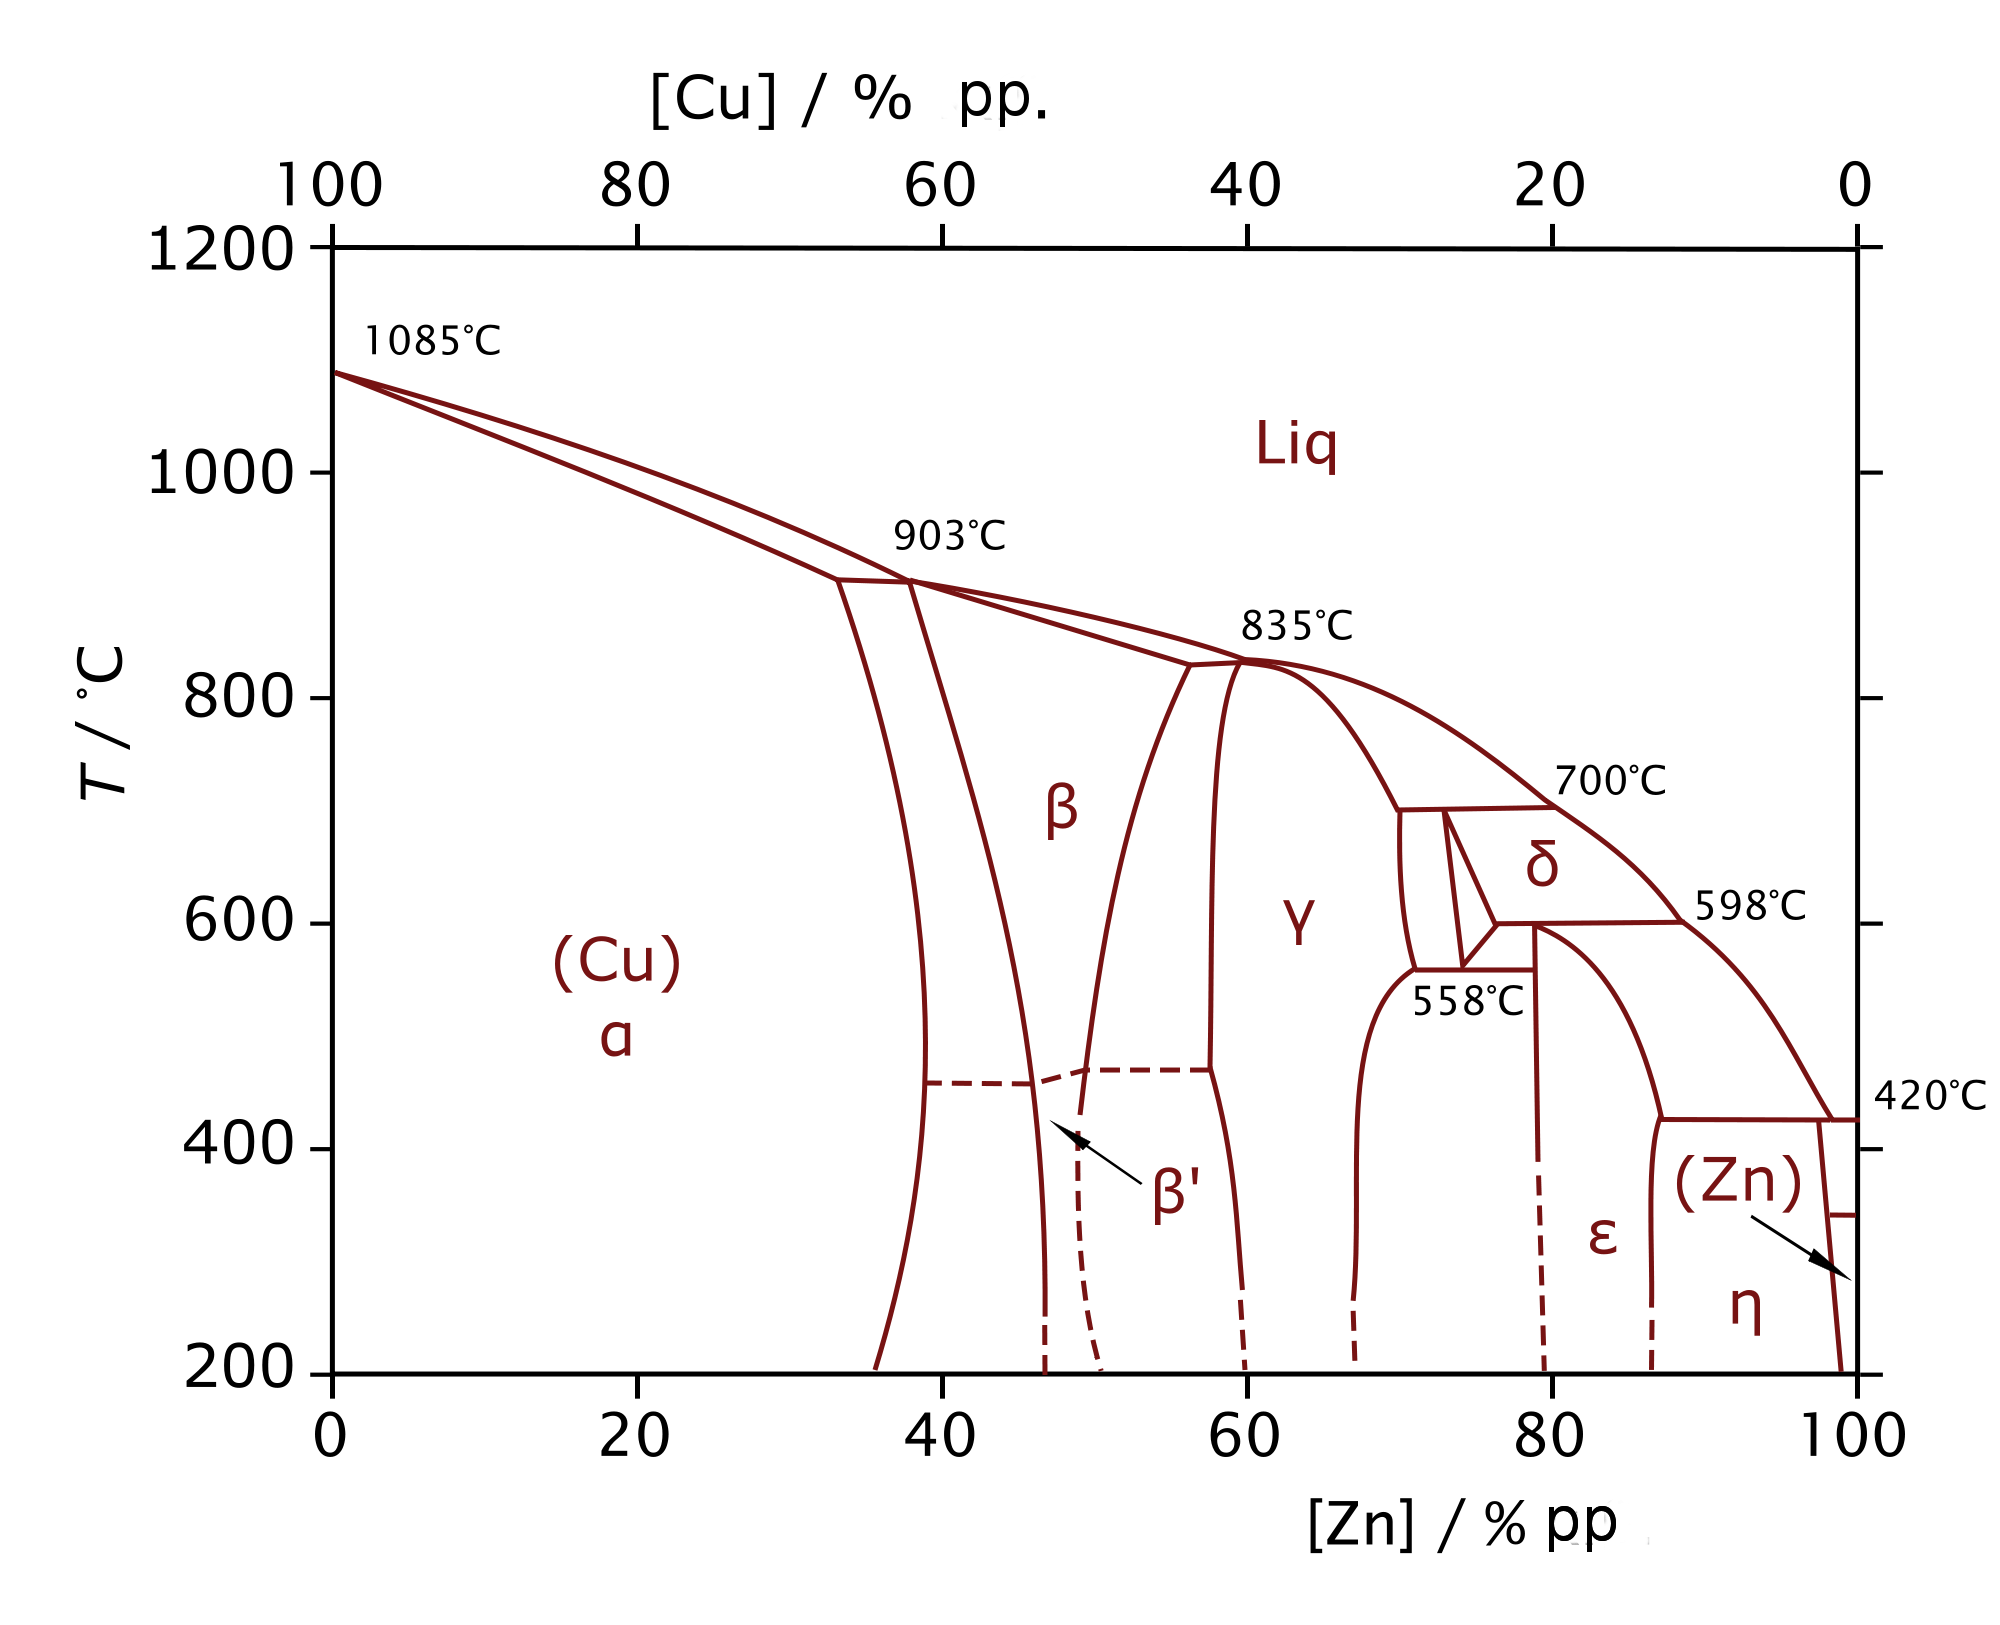
\includegraphics[width=0.8\textwidth]{img/intro/CuZn.png}
\begin{equation*}
 \beta \rightarrow B2 \rightarrow L2_1 \rightarrow 18R 
\end{equation*}
\end{frame}

%*************************
% ************************ 

\begin{frame}

\frametitle{$M_s$}

\begin{columns}
\column{0.4\textwidth}
 \begin{equation*}
\frac{e}{a} = 1+C_{Zn}+2C_{Al}
\end{equation*}
\begin{equation*}
M_s[K]=2686-6400C_{Zn}-9000C_{Al} \label{Ms} 
\end{equation*}
\begin{equation*}
     C_{Cu}+C_{Zn}+C_{Al}=1
\end{equation*}

\column{0.4\textwidth}

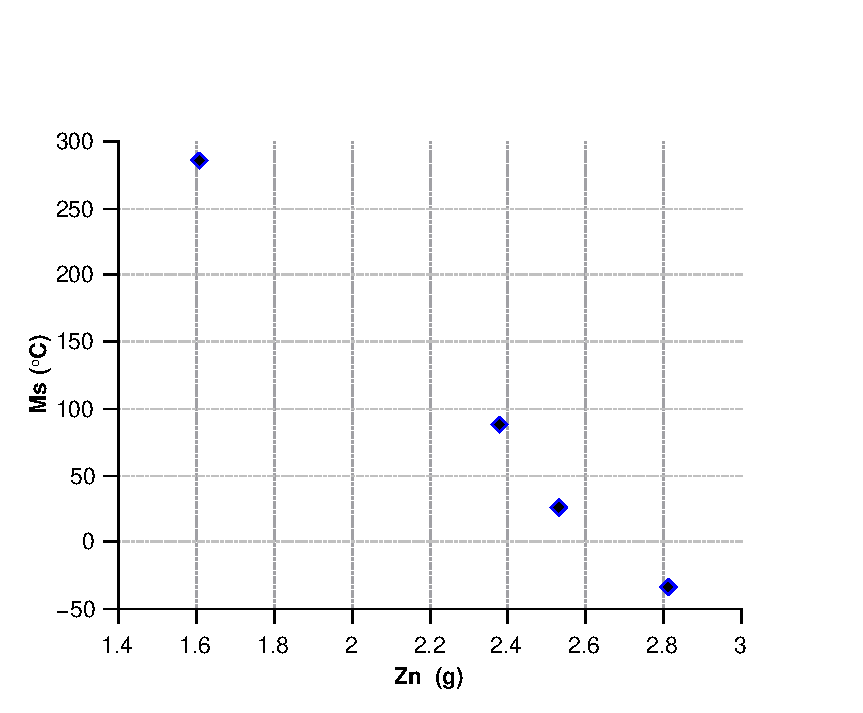
\includegraphics[width=\columnwidth]{img/intro/MsZn2.eps}

\end{columns}

\end{frame}

%*************************
% ************************ 
\begin{frame}
 
 Estrcturas celulares
 
\end{frame}




\begin{frame}
\frametitle{Esponjas metálicas}

\begin{multicols}{2}

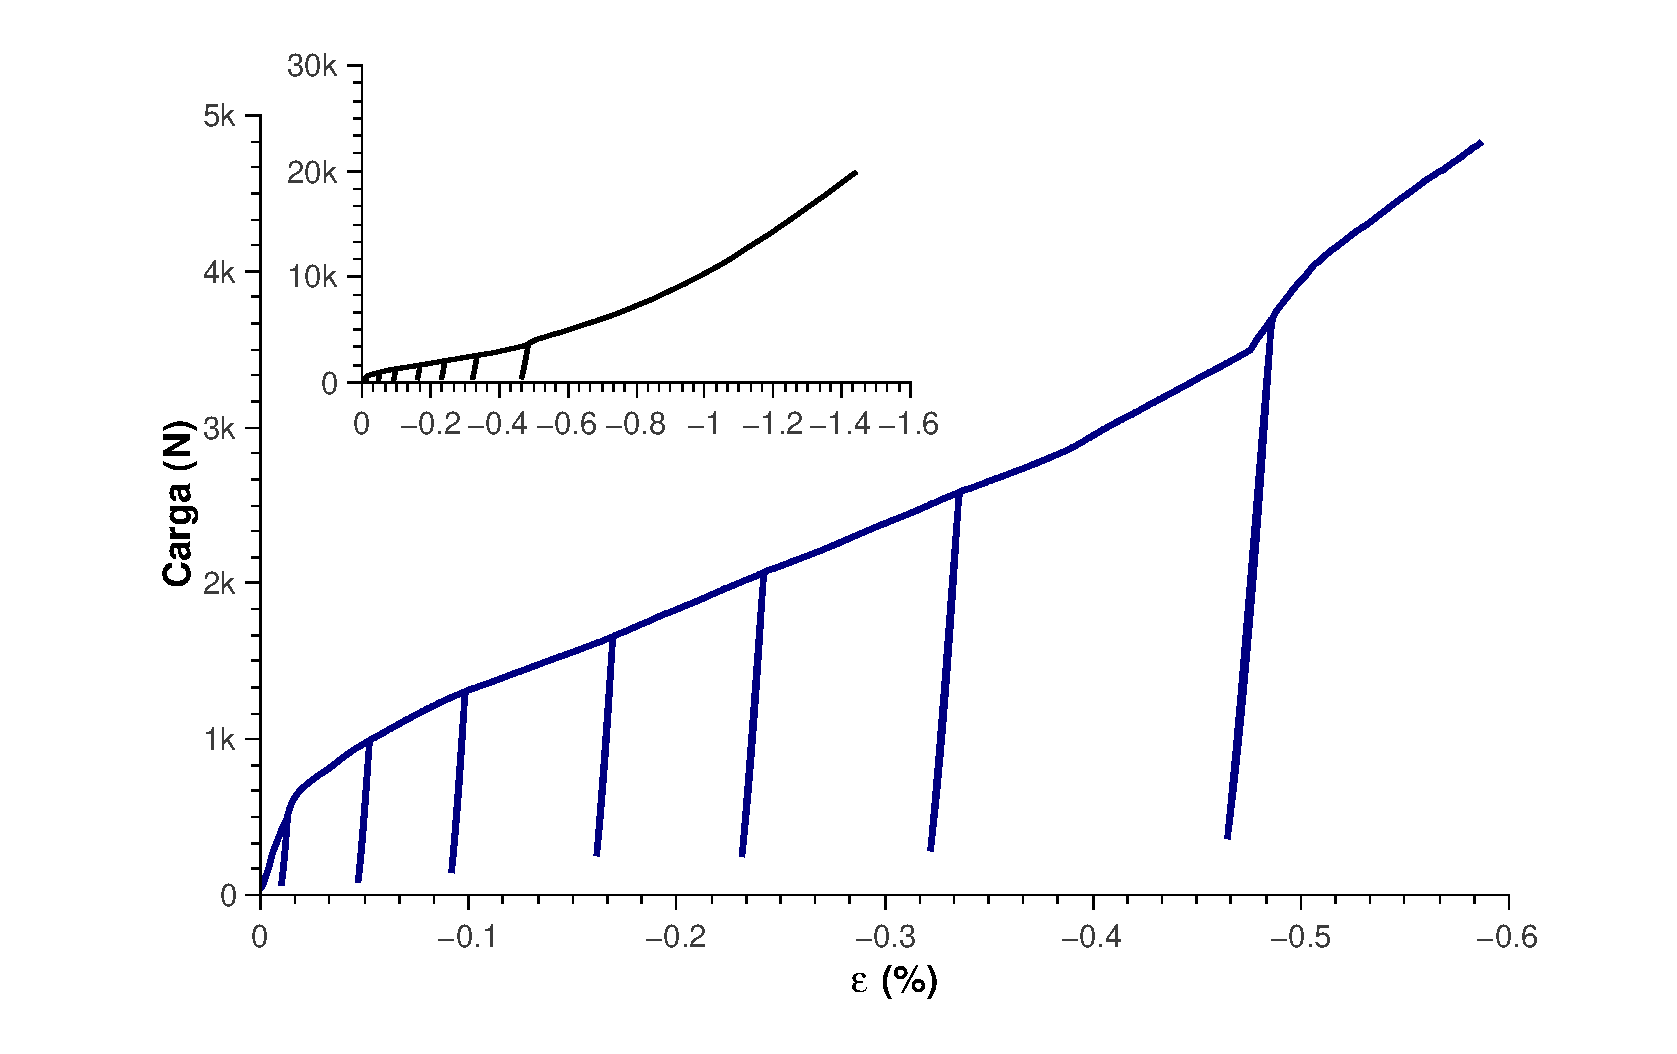
\includegraphics[width=0.5\textwidth]{img/intro/Cucompararesponja.eps}

\begin{itemize}
\small
 \item \alert<1>{Lineal-elástico $\rightarrow$ flexión de las paredes }
 \item \alert<2>{Colapso de la estructura $\rightarrow$ Fluencia o fractura}
 \item \alert<3>{Densificación  }
\end{itemize}

\end{multicols}
\alert<4>{Principal parámetro: Densidad específica $\frac{\rho^*}{\rho_s}$}

Principal forma de caracterizar las propiedades mecánicas 
\alert<5>{
\begin{equation*}
\frac{F^*}{F_s}=A \left(\frac{\rho^*}{\rho_s}\right)^n \label{props} 
\end{equation*}
}
sirve para rigidez de la estructura, tensión de colapso de la estructura $\sigma^{pl}$,
Deformación en bandas a $45 ^\circ$

\end{frame}

%*************************

\begin{frame}

\frametitle{Esponjas pseudoelásticas}

\begin{multicols}{2}

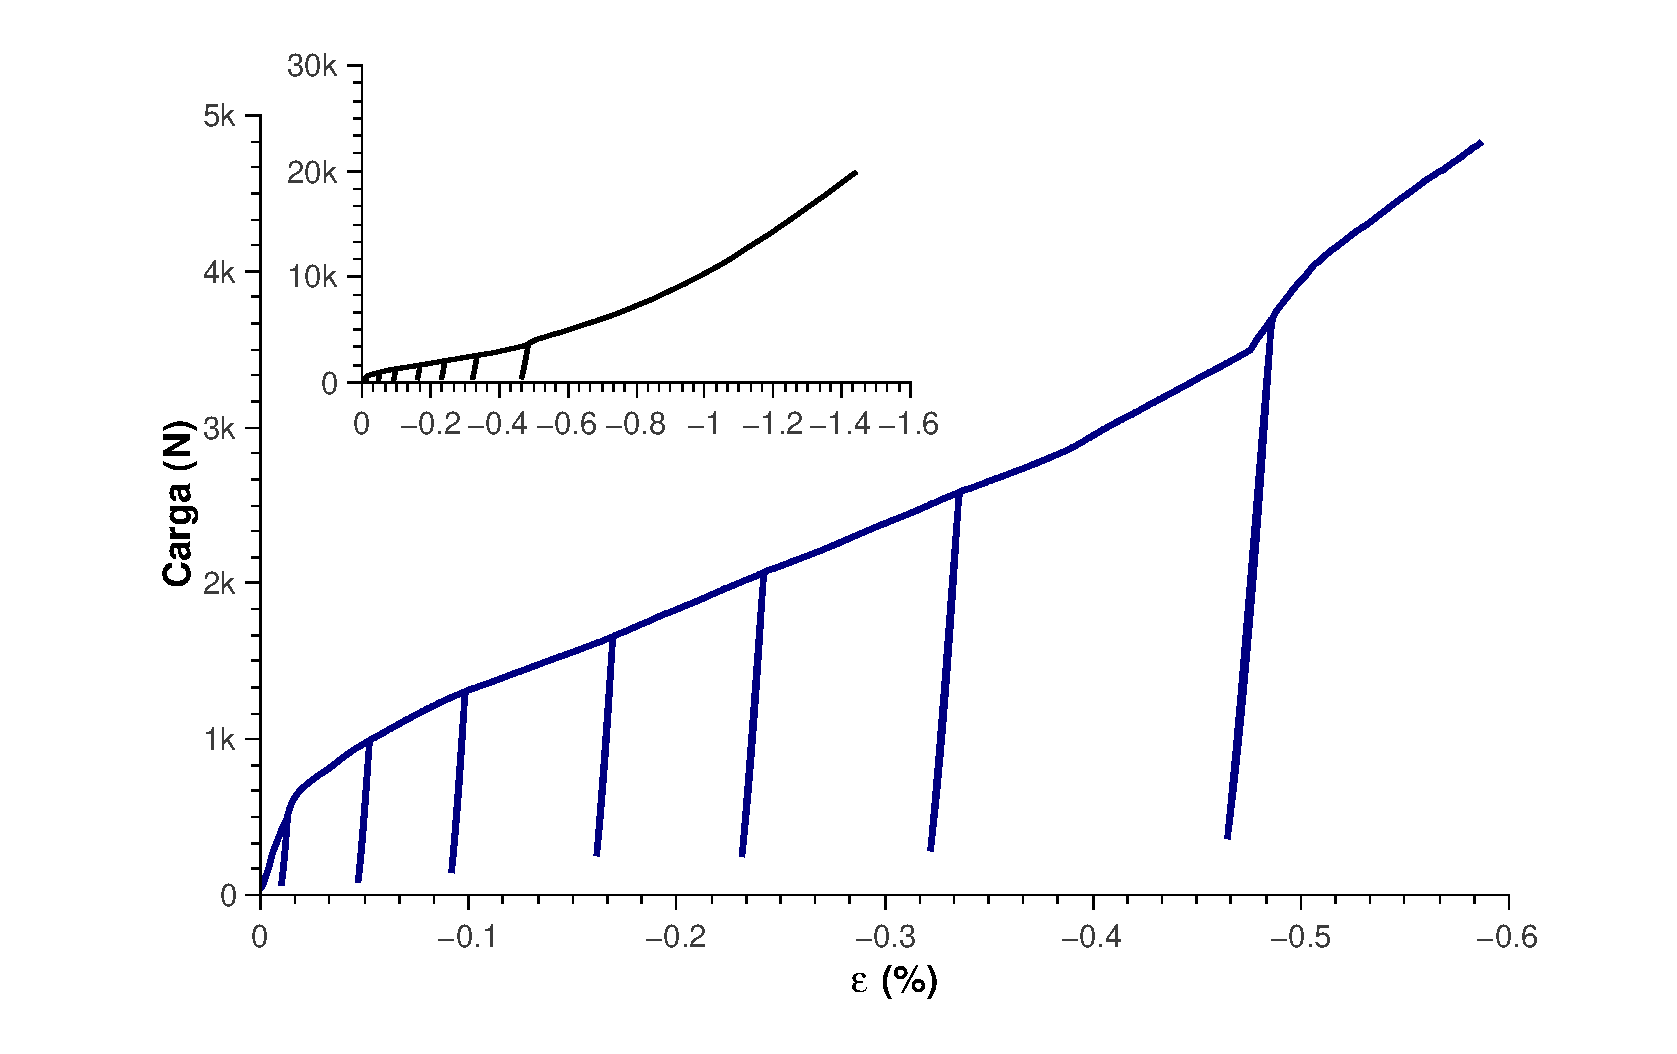
\includegraphics[width=0.5\textwidth]{img/intro/Cucompararesponja.eps}

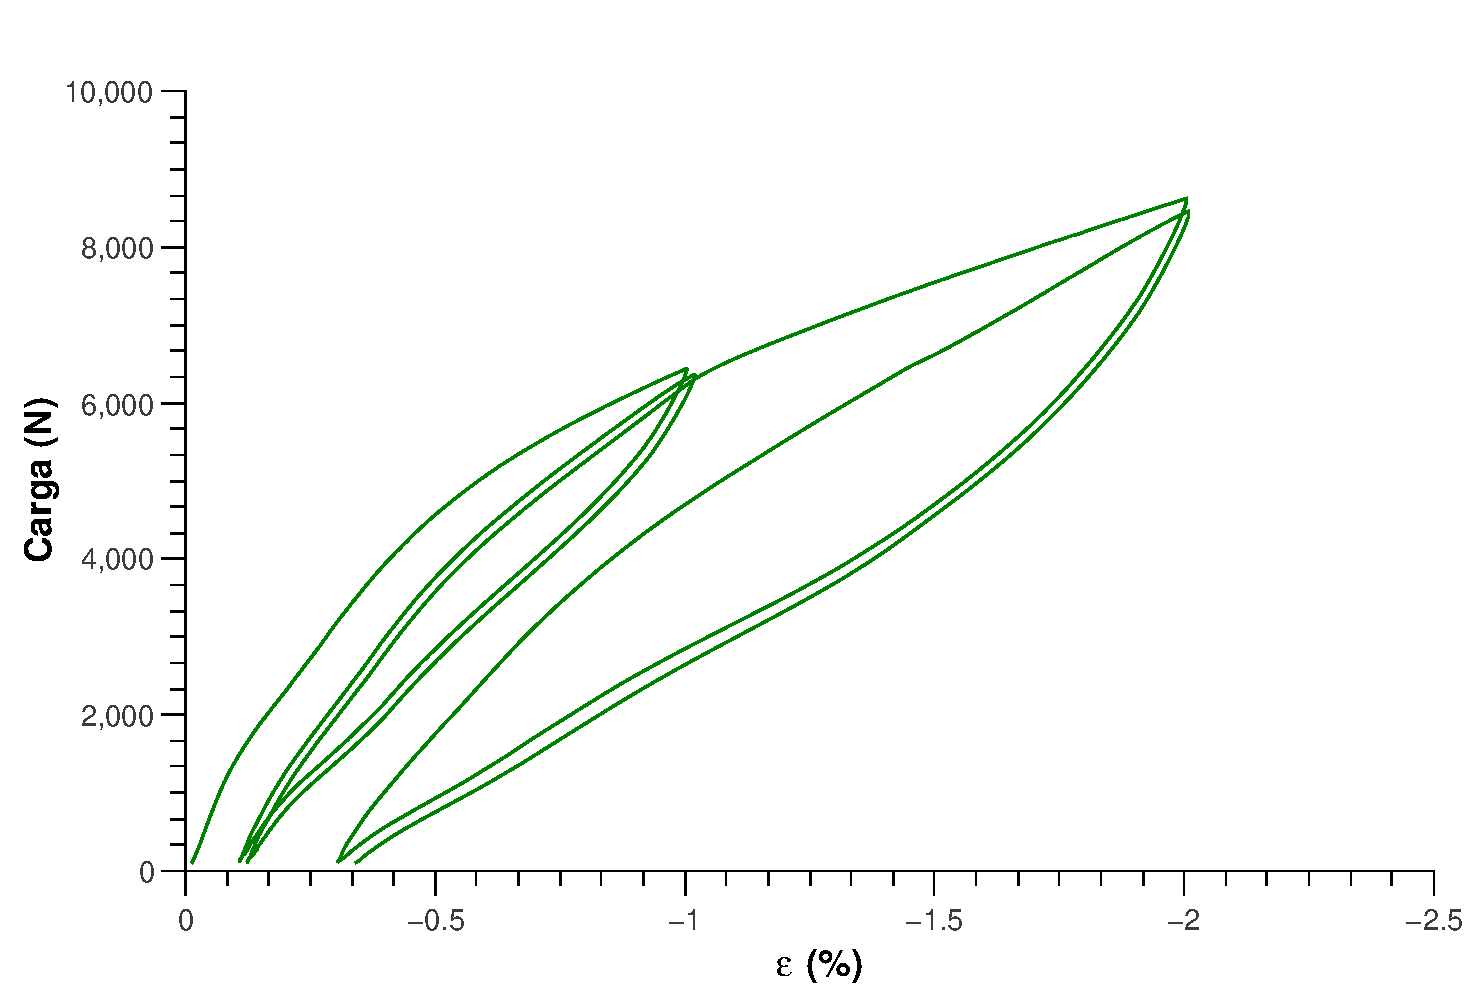
\includegraphics[width=0.5\textwidth]{img/intro/EsponjacompararCu.eps}

\end{multicols}


 \begin{itemize}
  \item \alert<1>{Gran capacidad de deformación}
  \item \alert<2>{Recuperación de la forma inicial}
  \item \alert<3>{Disipación de energía por el efecto pseudoelástico}
 \end{itemize}

\end{frame}

%*************************

% 
% \begin{frame}
%  \begin{itemize}
%   \item Memoria de forma
%   
%  
%  \end{itemize}
%  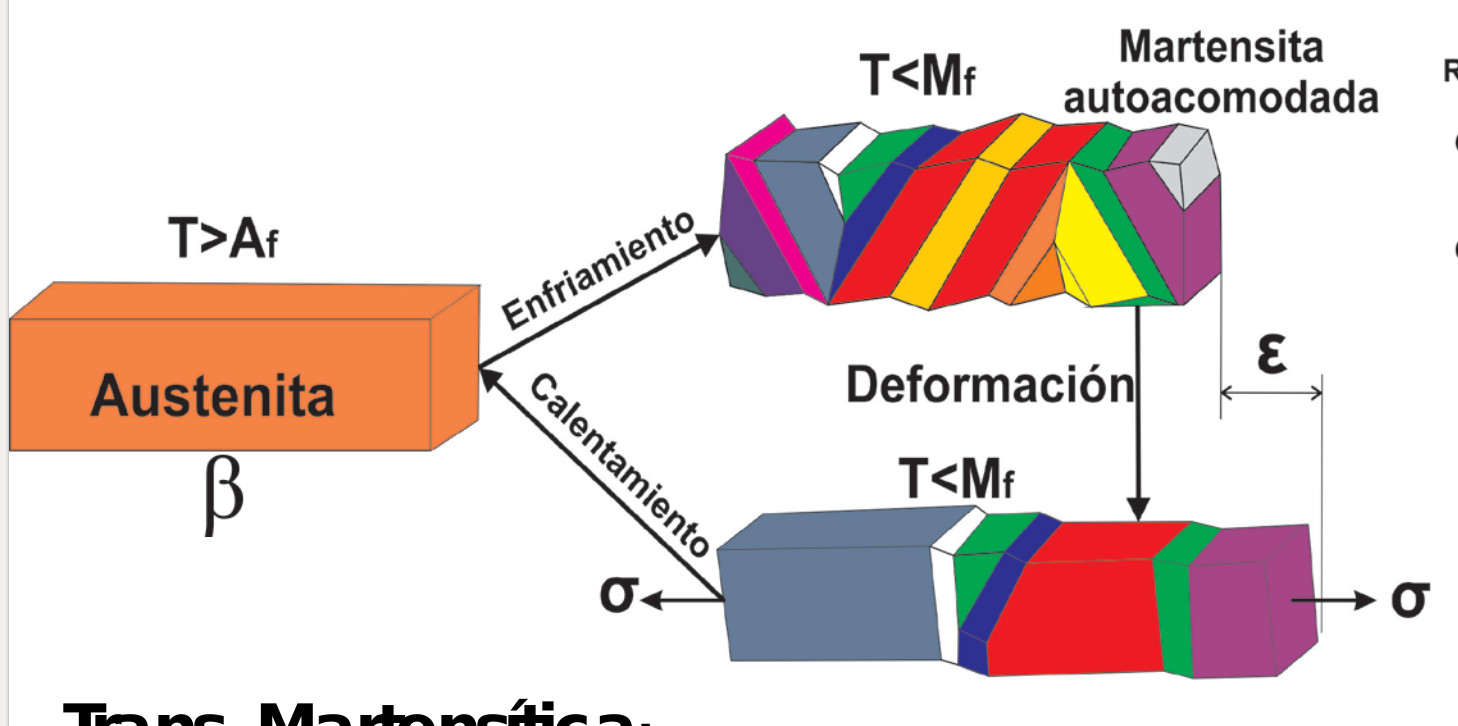
\includegraphics[width=0.8\textwidth]{img/intro/memoria.jpg}
% \end{frame}

% ******************

\begin{frame}

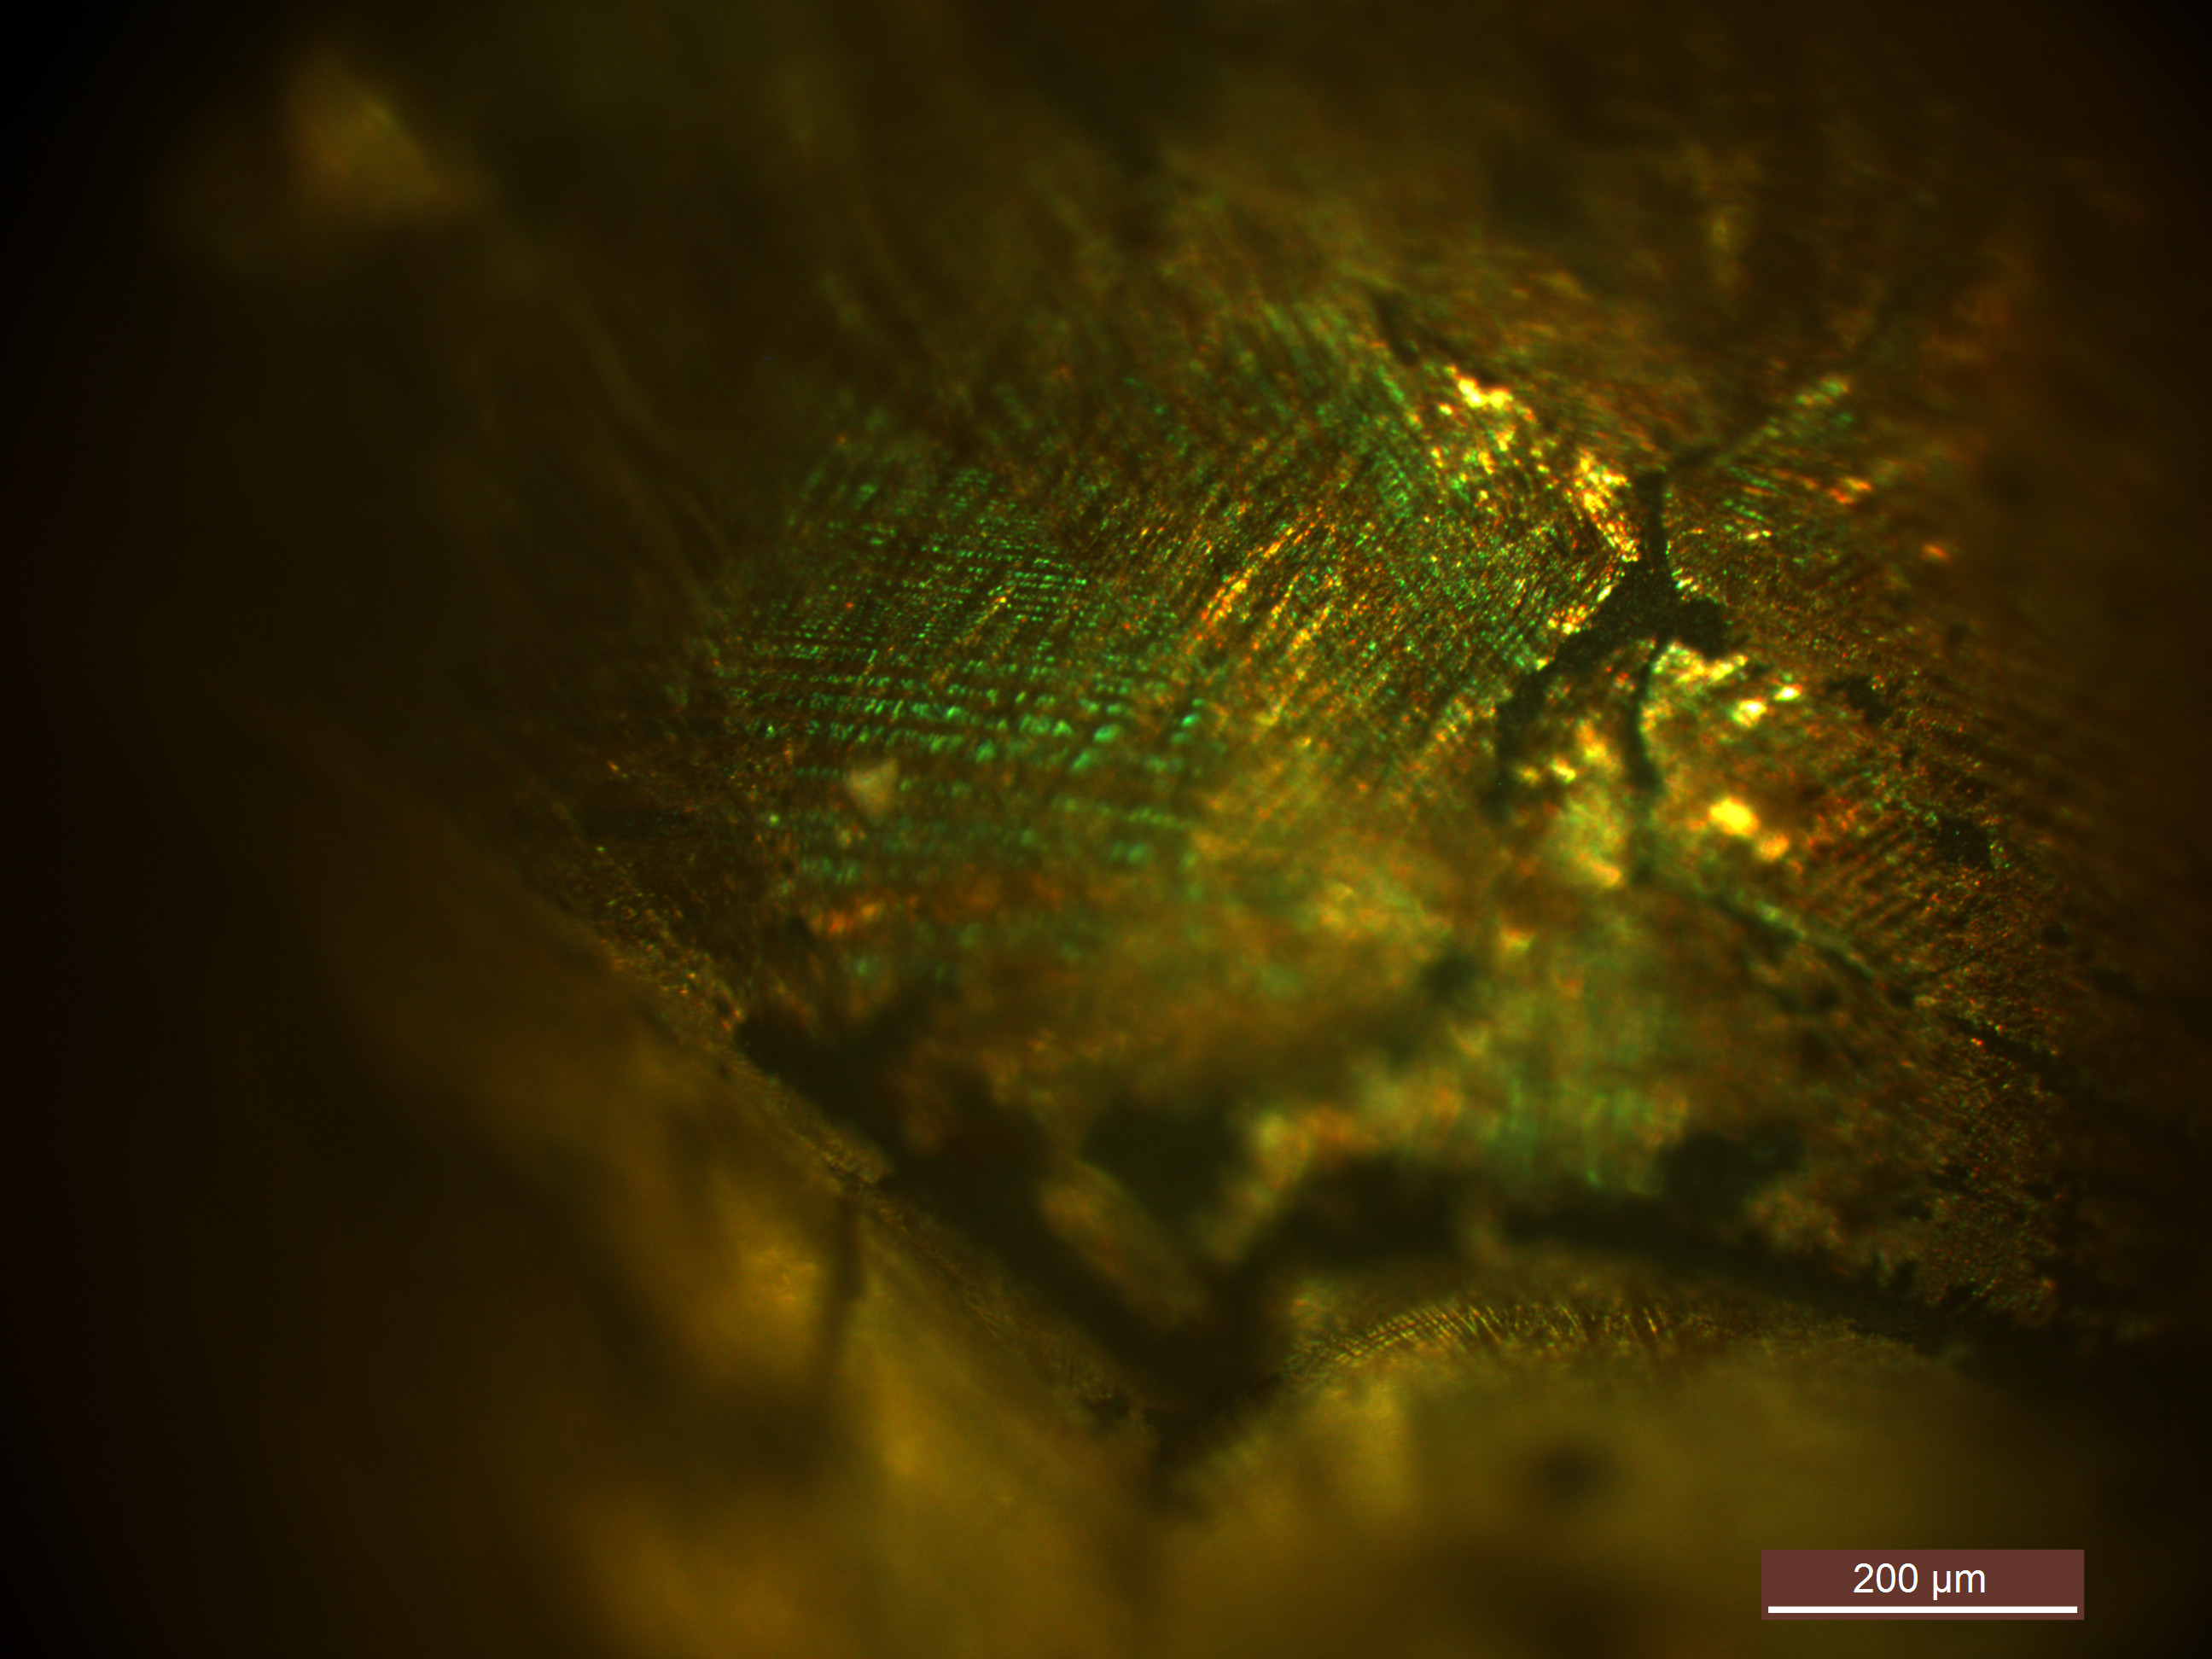
\includegraphics[width=0.4\textwidth]{img/intro/EspAMicro4.jpg}

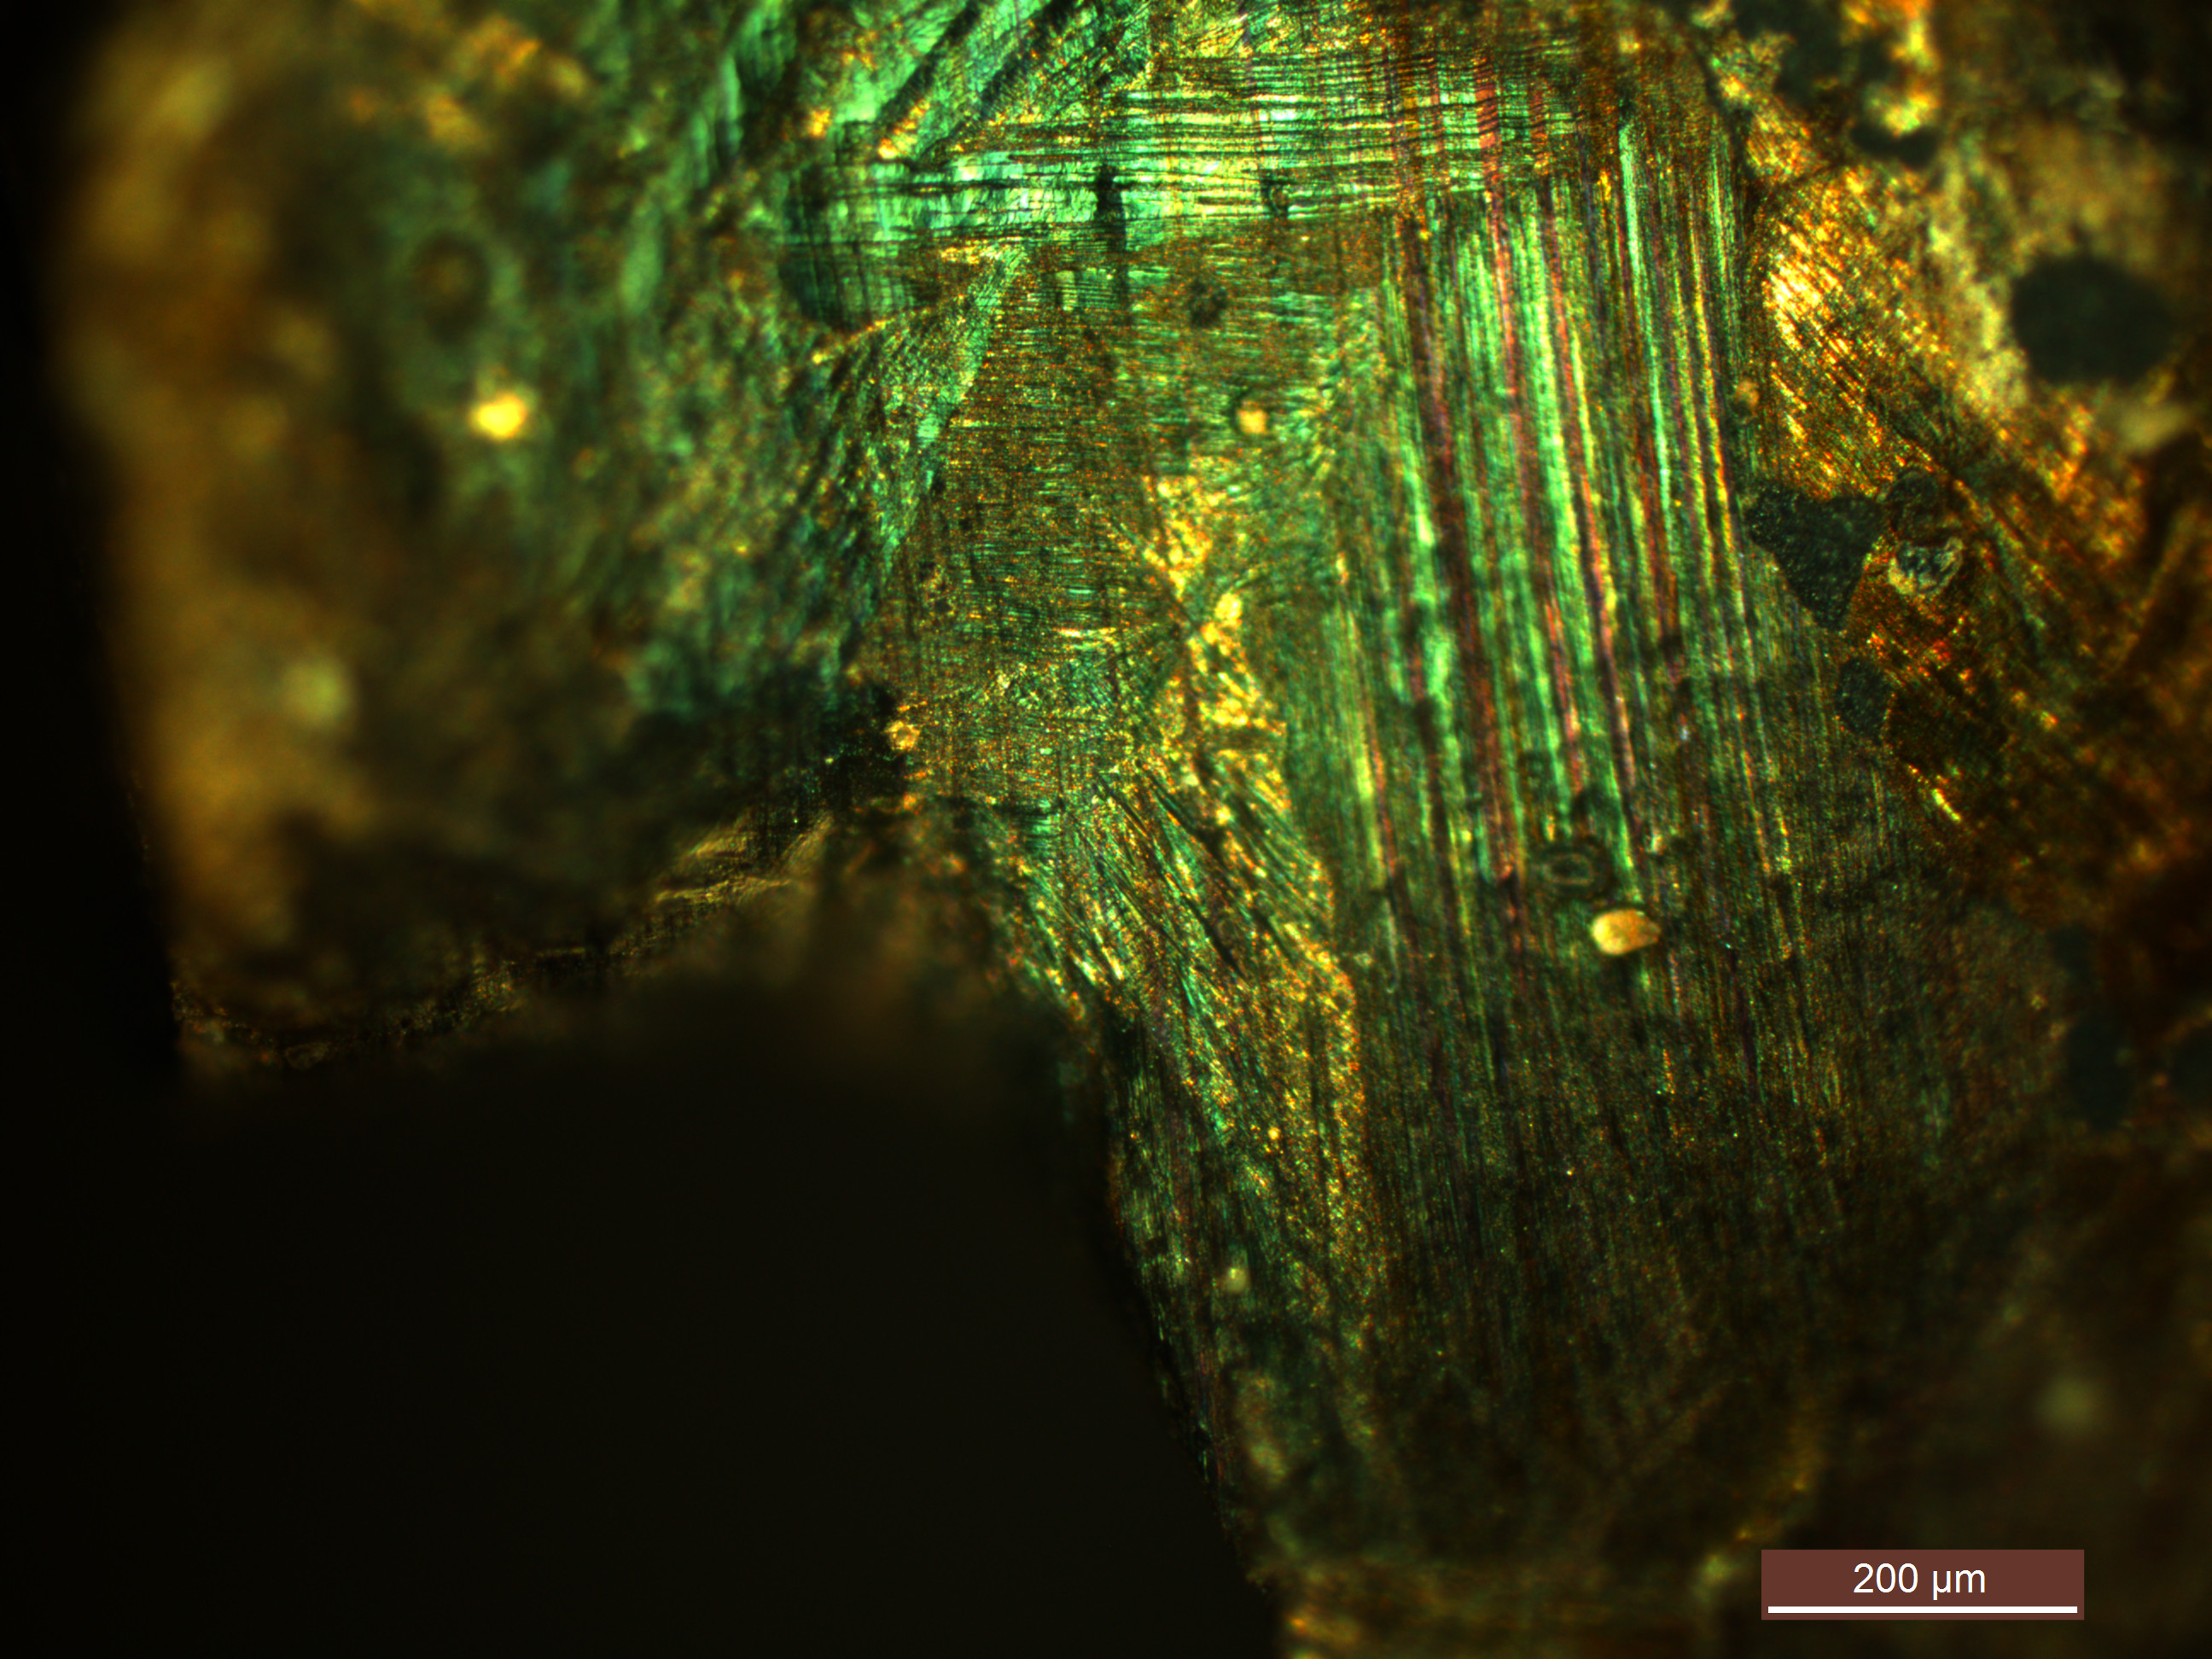
\includegraphics[width=0.4\textwidth]{img/intro/EspAMicro2.jpg}
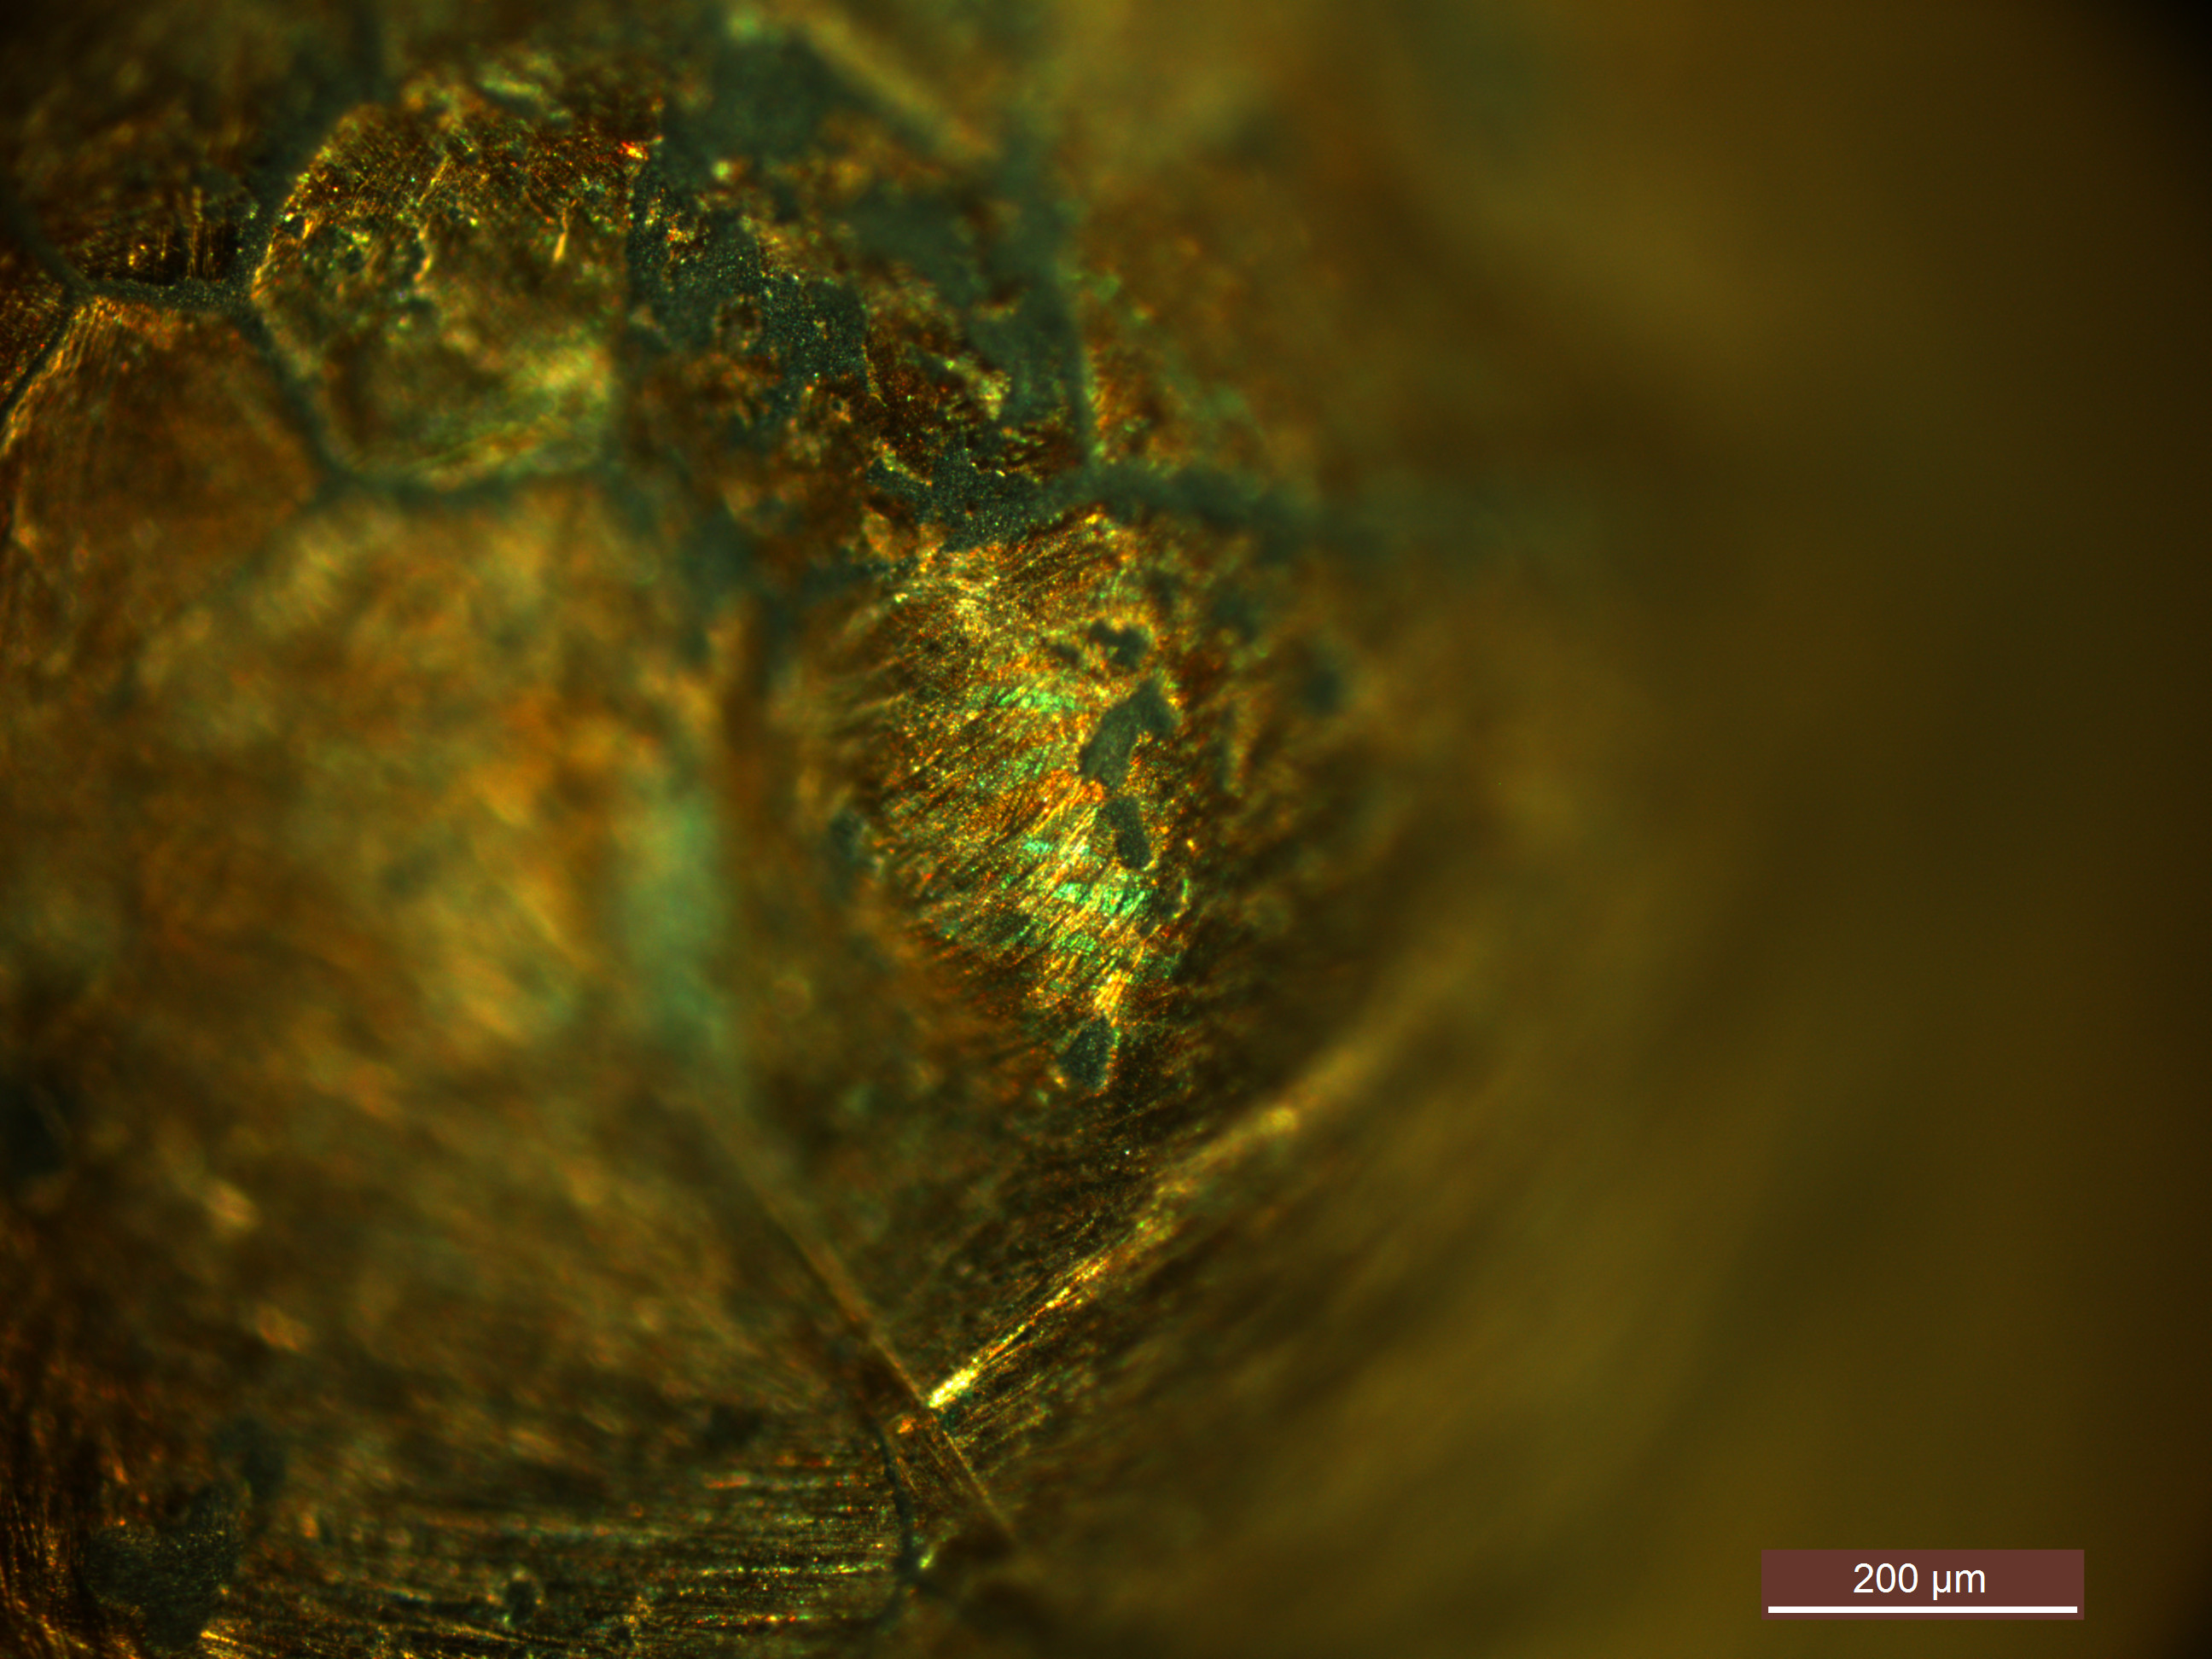
\includegraphics[width=0.4\textwidth]{img/intro/EspAMicro3.jpg}
 
\end{frame}
%%%%%%%%%%%%%%%%%%%%%%%%%%%%%%%%%%%%%%%%%%%%%%%%%%%%%%%%%%%%%%%%%%%%%%%%%%%%%%%%%%%%%%%%%%%%%%%%%55
% \begin{frame}
% Anisotropía elástica lleva a fisuras intergranulares 
% \end{frame}



% ******************

% \begin{frame}
%  Esponjas pseudoelásticas
% \end{frame}

% ******************************************************************************************************************************

\begin{frame}
 
 \frametitle{Preparación de la aleación}
 
 \begin{itemize}
 \item[$\circ$] Cu: $50 \%$ ácido nítrico (al $65 \%$) - $50 \%$ agua
 \item[$\circ$] Zn: $60 \%$ ácido nítrico (al $65 \%$) - $40 \%$ agua
 \item[$\circ$] Al: $60 \%$ agua - $30 \%$ ácido clorhídrico (al 37 \%) - $10 \%$ ácido fluorhídrico (al $48 \%$)
\end{itemize}
\end{frame}

\begin{frame}
\frametitle{Método de fabricación de esponjas pseudoelásticas}
\begin{center}
\begin{multicols}{4}
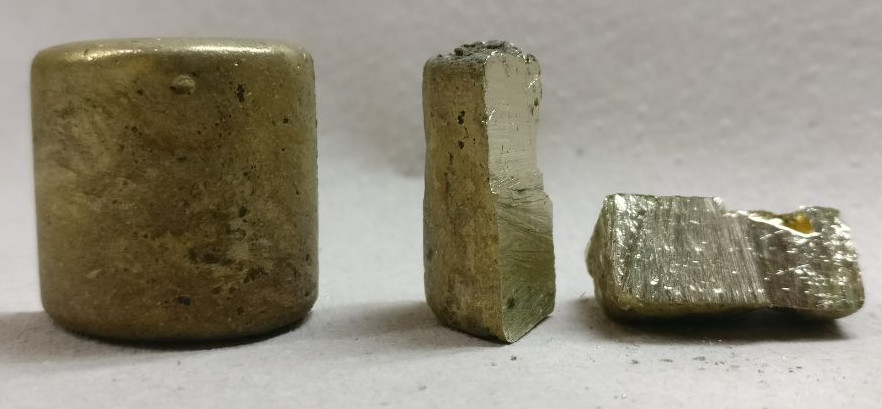
\includegraphics[width=0.25\textwidth]{img/proceso/lingote.jpg}



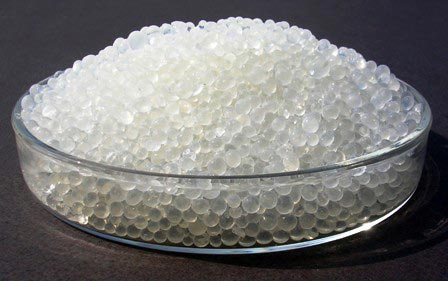
\includegraphics[width=0.25\textwidth]{img/proceso/silica.jpg}


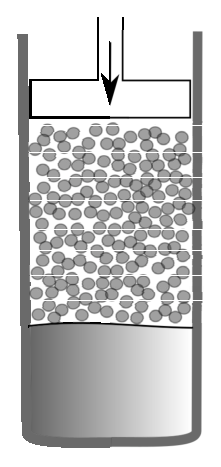
\includegraphics[width=0.15\textwidth]{img/proceso/proceso1.eps}

%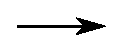
\includegraphics[width=0.05\textwidth]{img/proceso/flecha.eps}

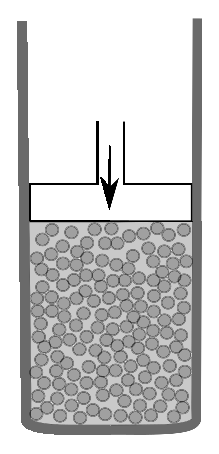
\includegraphics[width=0.15\textwidth]{img/proceso/proceso2.eps}
\vfill
%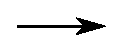
\includegraphics[width=0.05\textwidth]{img/proceso/flecha.eps}

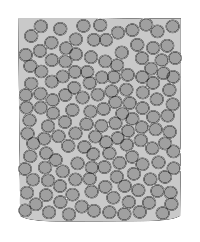
\includegraphics[width=0.15\textwidth]{img/proceso/proceso3.eps}
\end{multicols}

\begin{multicols}{3}

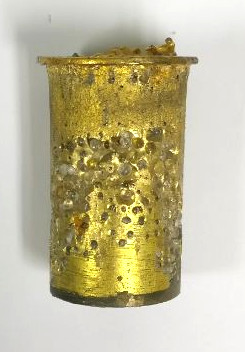
\includegraphics[width=0.25\textwidth]{img/proceso/proceso1.jpg}

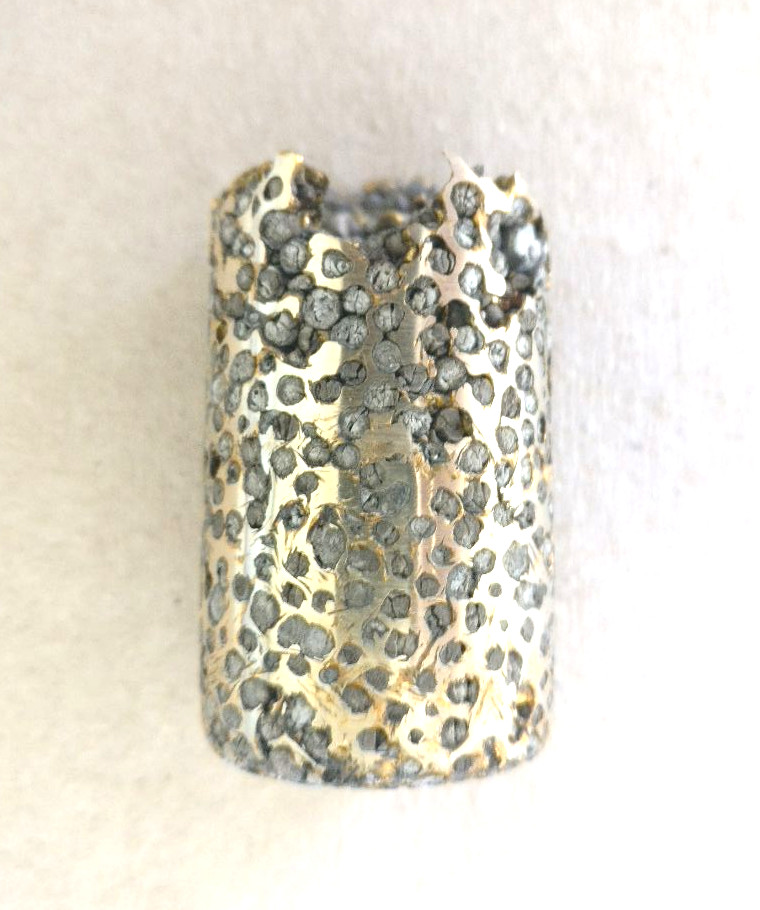
\includegraphics[width=0.25\textwidth]{img/proceso/proceso2.jpg}

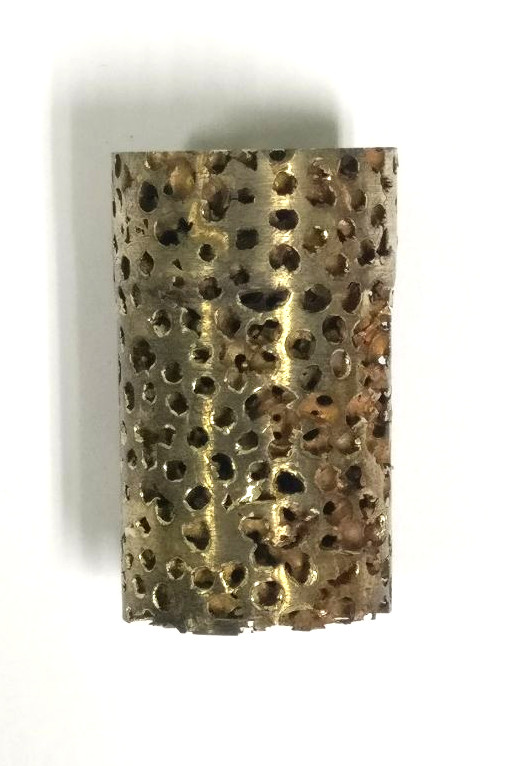
\includegraphics[width=0.25\textwidth]{img/proceso/proceso3.jpg}
\end{multicols}

\end{center}
\end{frame}
%%%%%%%%%%%%%%%%%%%%%%%%%%%%%%%%%%%%%%%%%%%%%%%%%%%%%%%%%%%%%%%%%%%%%%

\begin{frame}
\frametitle{Medición de la $M_s$}

 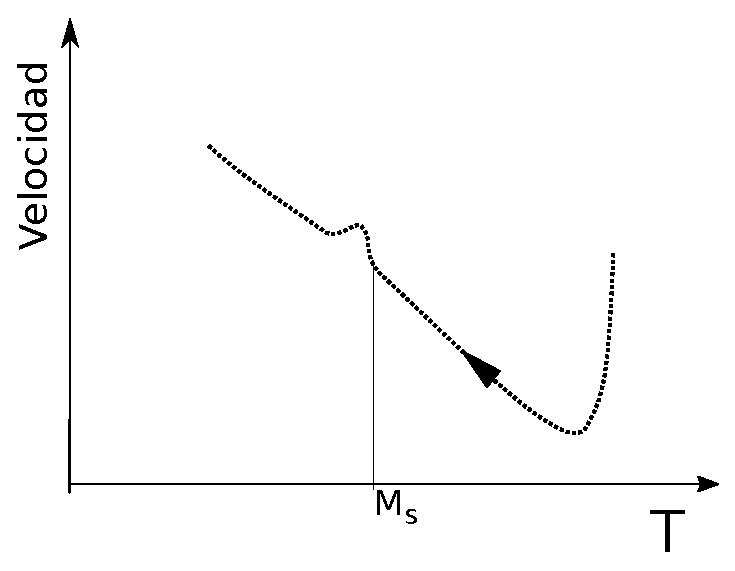
\includegraphics[width=0.5\textwidth]{img/proceso/Ms.eps}

\end{frame}

%%%%%%%%%%%%%%%%%%%%%%%%%%%%%%%%%%%%%%%%%%%%%%%%%%%%%%%%%%%%%%%%%%%%%%




\section{Motivación}

\begin{frame}
\frametitle{motivación}


%\begin{multicols}{2}
\begin{center}

\includegraphics[width=0.4\textwidth]{img/tamgrano/Esponjacompleta1.eps}
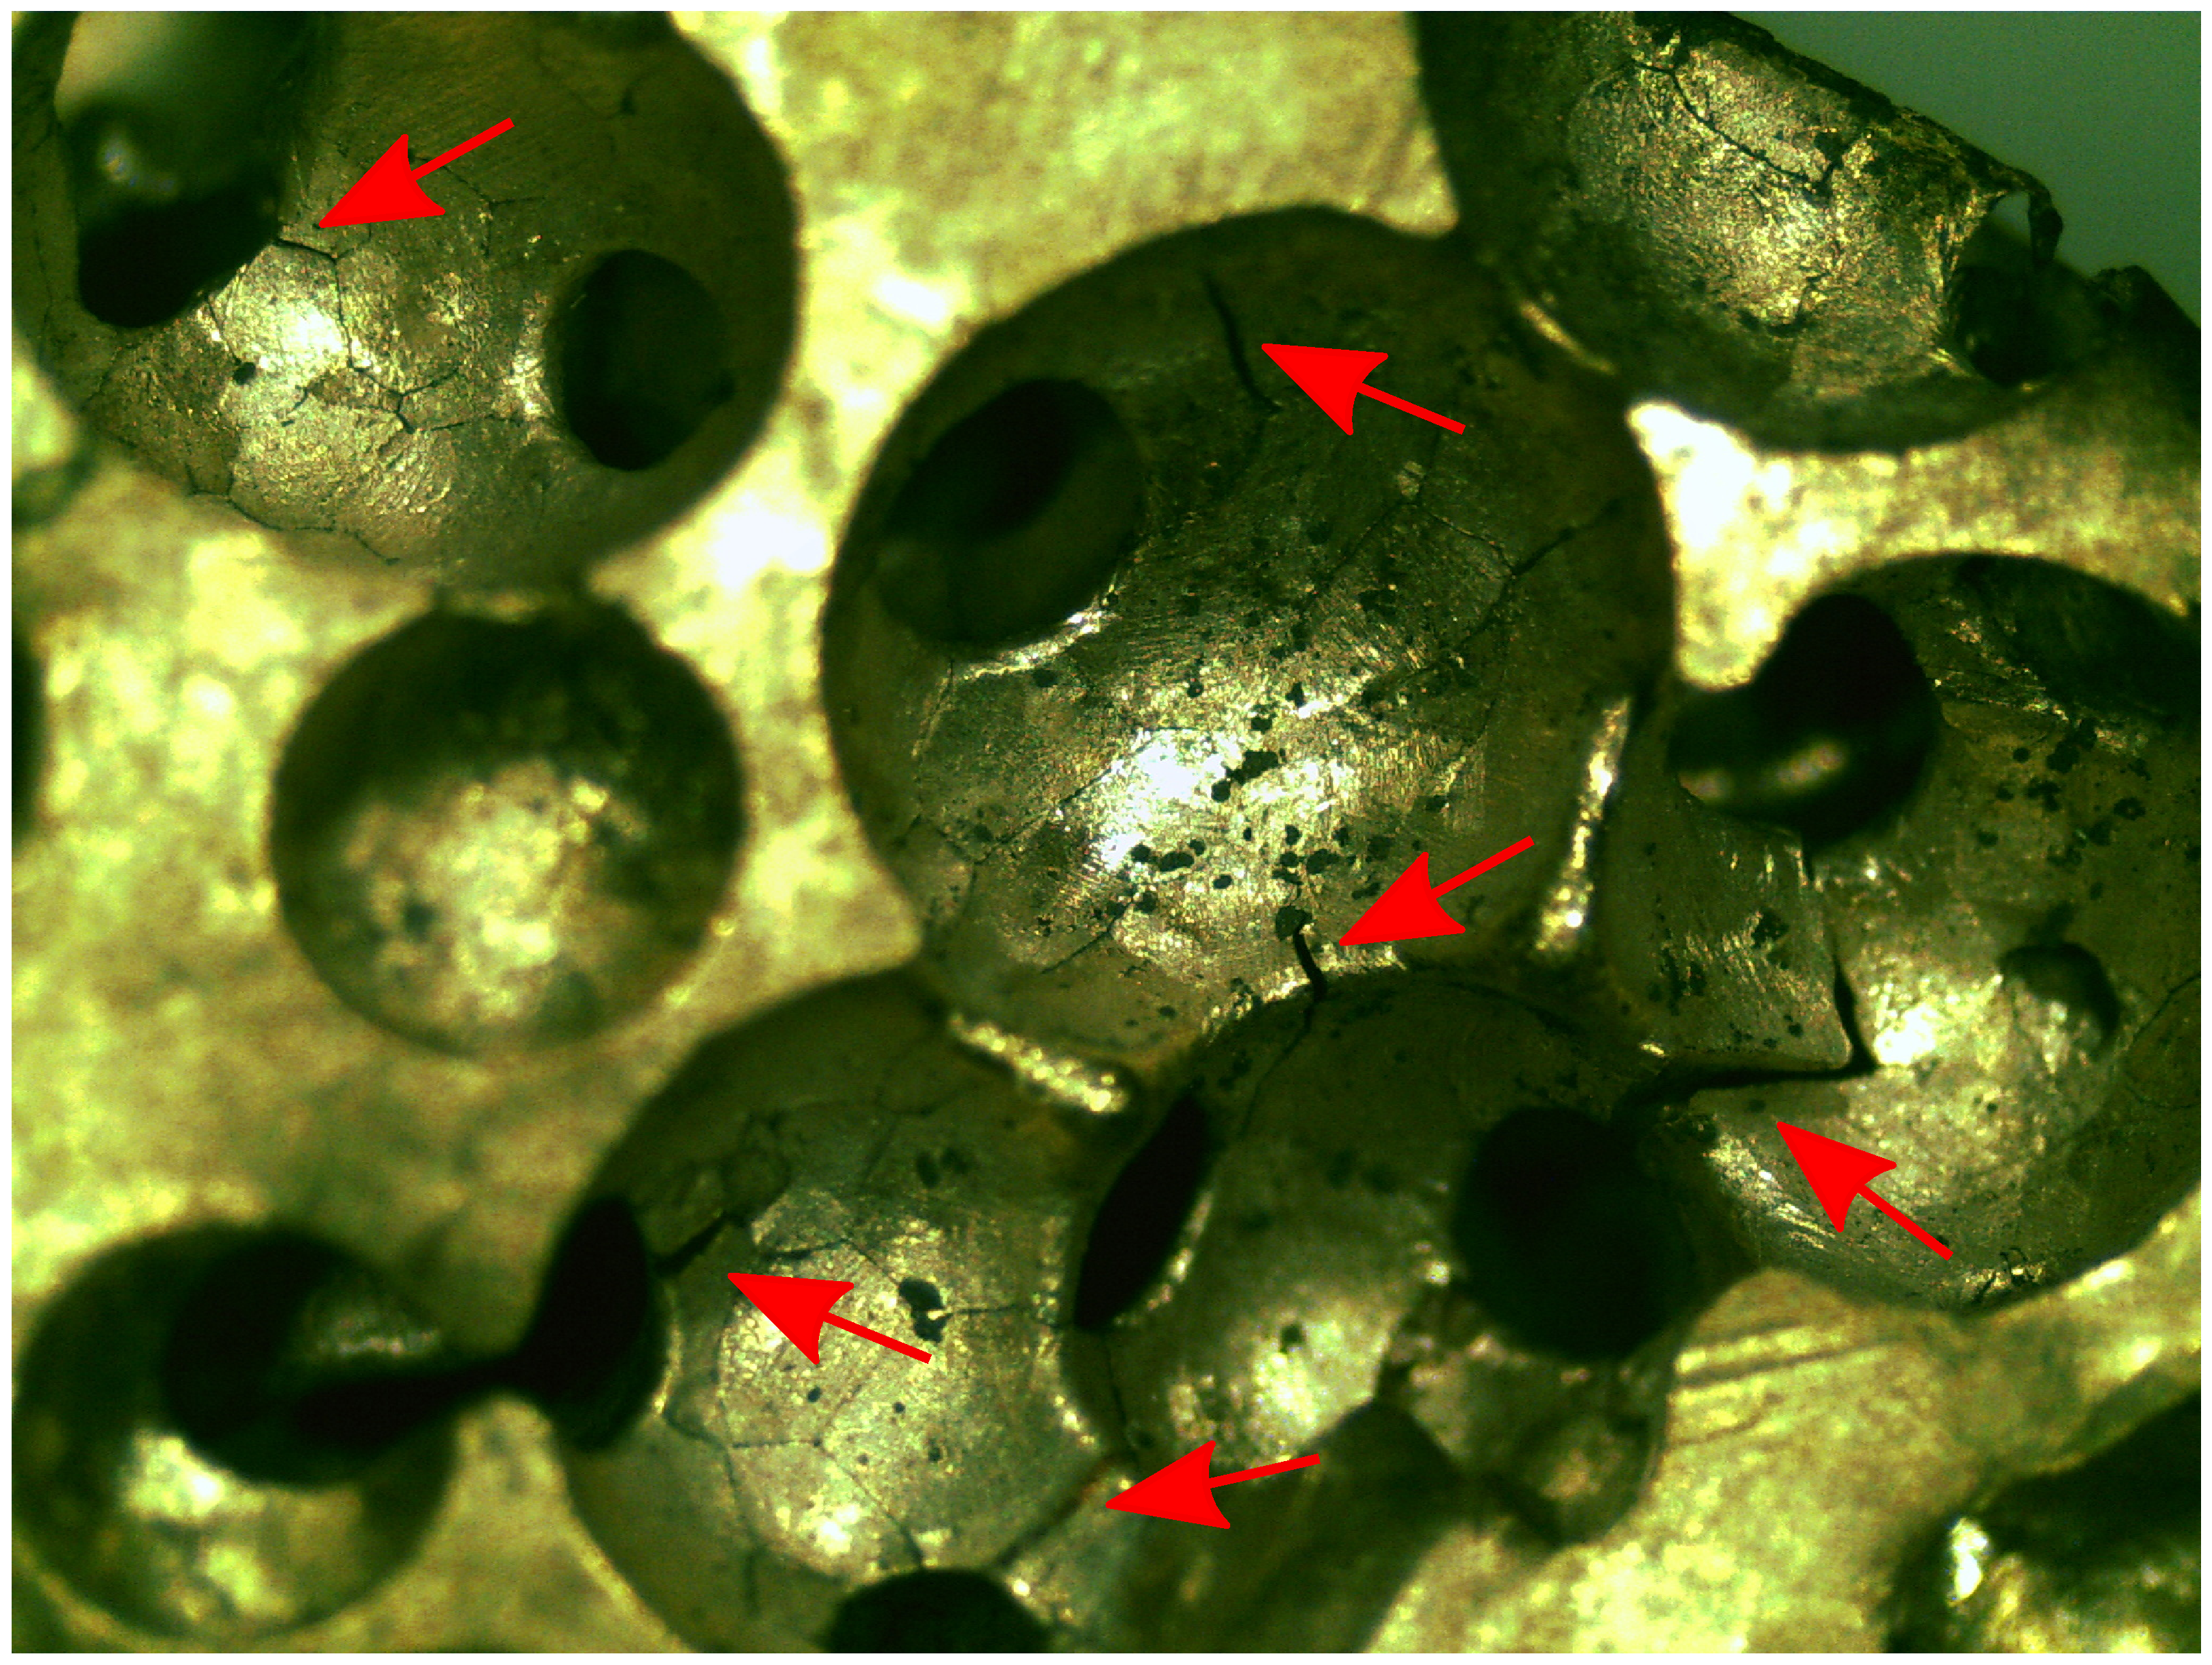
\includegraphics[width=0.5\textwidth]{img/tamgrano/Fisuras.eps}

\end{center}
%\end{multicols}

\alert<1>{Ensayos de distintas esponjas} $\rightarrow$ \alert<2>{fisuras intergranulares} $\rightarrow$ \alert<3>{Modificar tamaño de grano}
 
\alert<4>{Comportamiento mecánico de la estructura + transformaciones $=$ Muy complejo!!} $\rightarrow$ \alert<5>{buscamos método sencillo para entender lo que sucede y poder seguir la integridad estructural de la esponja.} 
\end{frame}


\subsection{Tamaño de grano}

% ******************
% \begin{frame}
%  Introducción fractura intergranular
% \end{frame}

% ******************

\begin{frame}
 \frametitle{Disminución tamaño de grano}

\begin{small}
\begin{tabular}{@{}lllllll@{}}  \toprule
Muestra            & $Cu-Zn-Al (g)$ &   $\% pp$ $AlB_2$ & Método & Horno \\ \midrule
\alert<1>{Botón 1} & 18,866         & 0,005             & 1      & Inducción\\
\alert<2>{Botón 2} & 18,564         & 0,5               & 1      &Resistivo\\
\alert<3>{Botón 3} & 14,129         & 0,5               & 2     &Resistivo \\
\alert<4>{Botón 4} & 18,383         & 0,5               & 2     & Resistivo \\
% Clavo 1 & 8 & - & - & 0,5 & 0,5 & III & Resistivo \\
% Clavo 2 & 8 & - & - & 0,05 & 0,05 &III & Resistivo \\
% Clavo 3 & 8 & - & - & - & - &  IV & Resistivo \\
% Clavo 4 & 8 & - & - & 0,005 & 0,005 &IV & Resistivo \\
\bottomrule
\end{tabular}
\end{small}

\begin{description}
\alert<1,2>{\item[Método 1:] Aleación $+$ $AlB_2$ papel aluminio $+$ $Cu$} 
\alert<3,4>{\item[Método 2:] Aleación $+$ $AlB_2$ $\rightarrow$  prensado de pastillas}
\end{description}

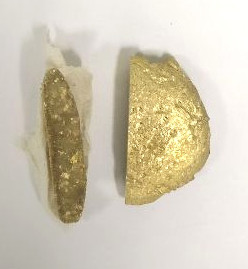
\includegraphics[width=0.16\textwidth]{img/proceso/boton.jpg}
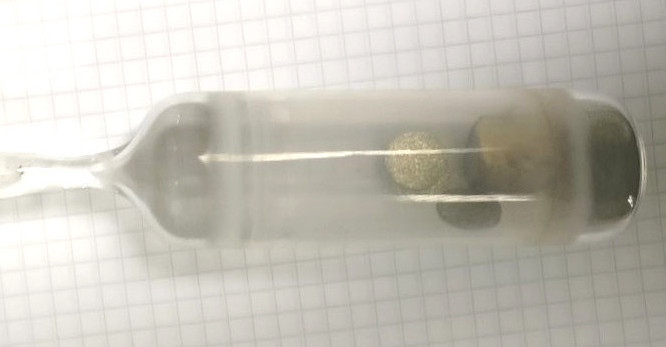
\includegraphics[width=0.33\textwidth]{img/proceso/ampolla.jpg}
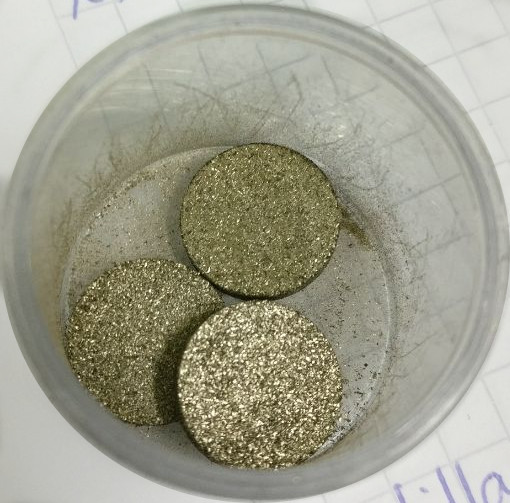
\includegraphics[width=0.175\textwidth]{img/proceso/PastViruta.jpg}
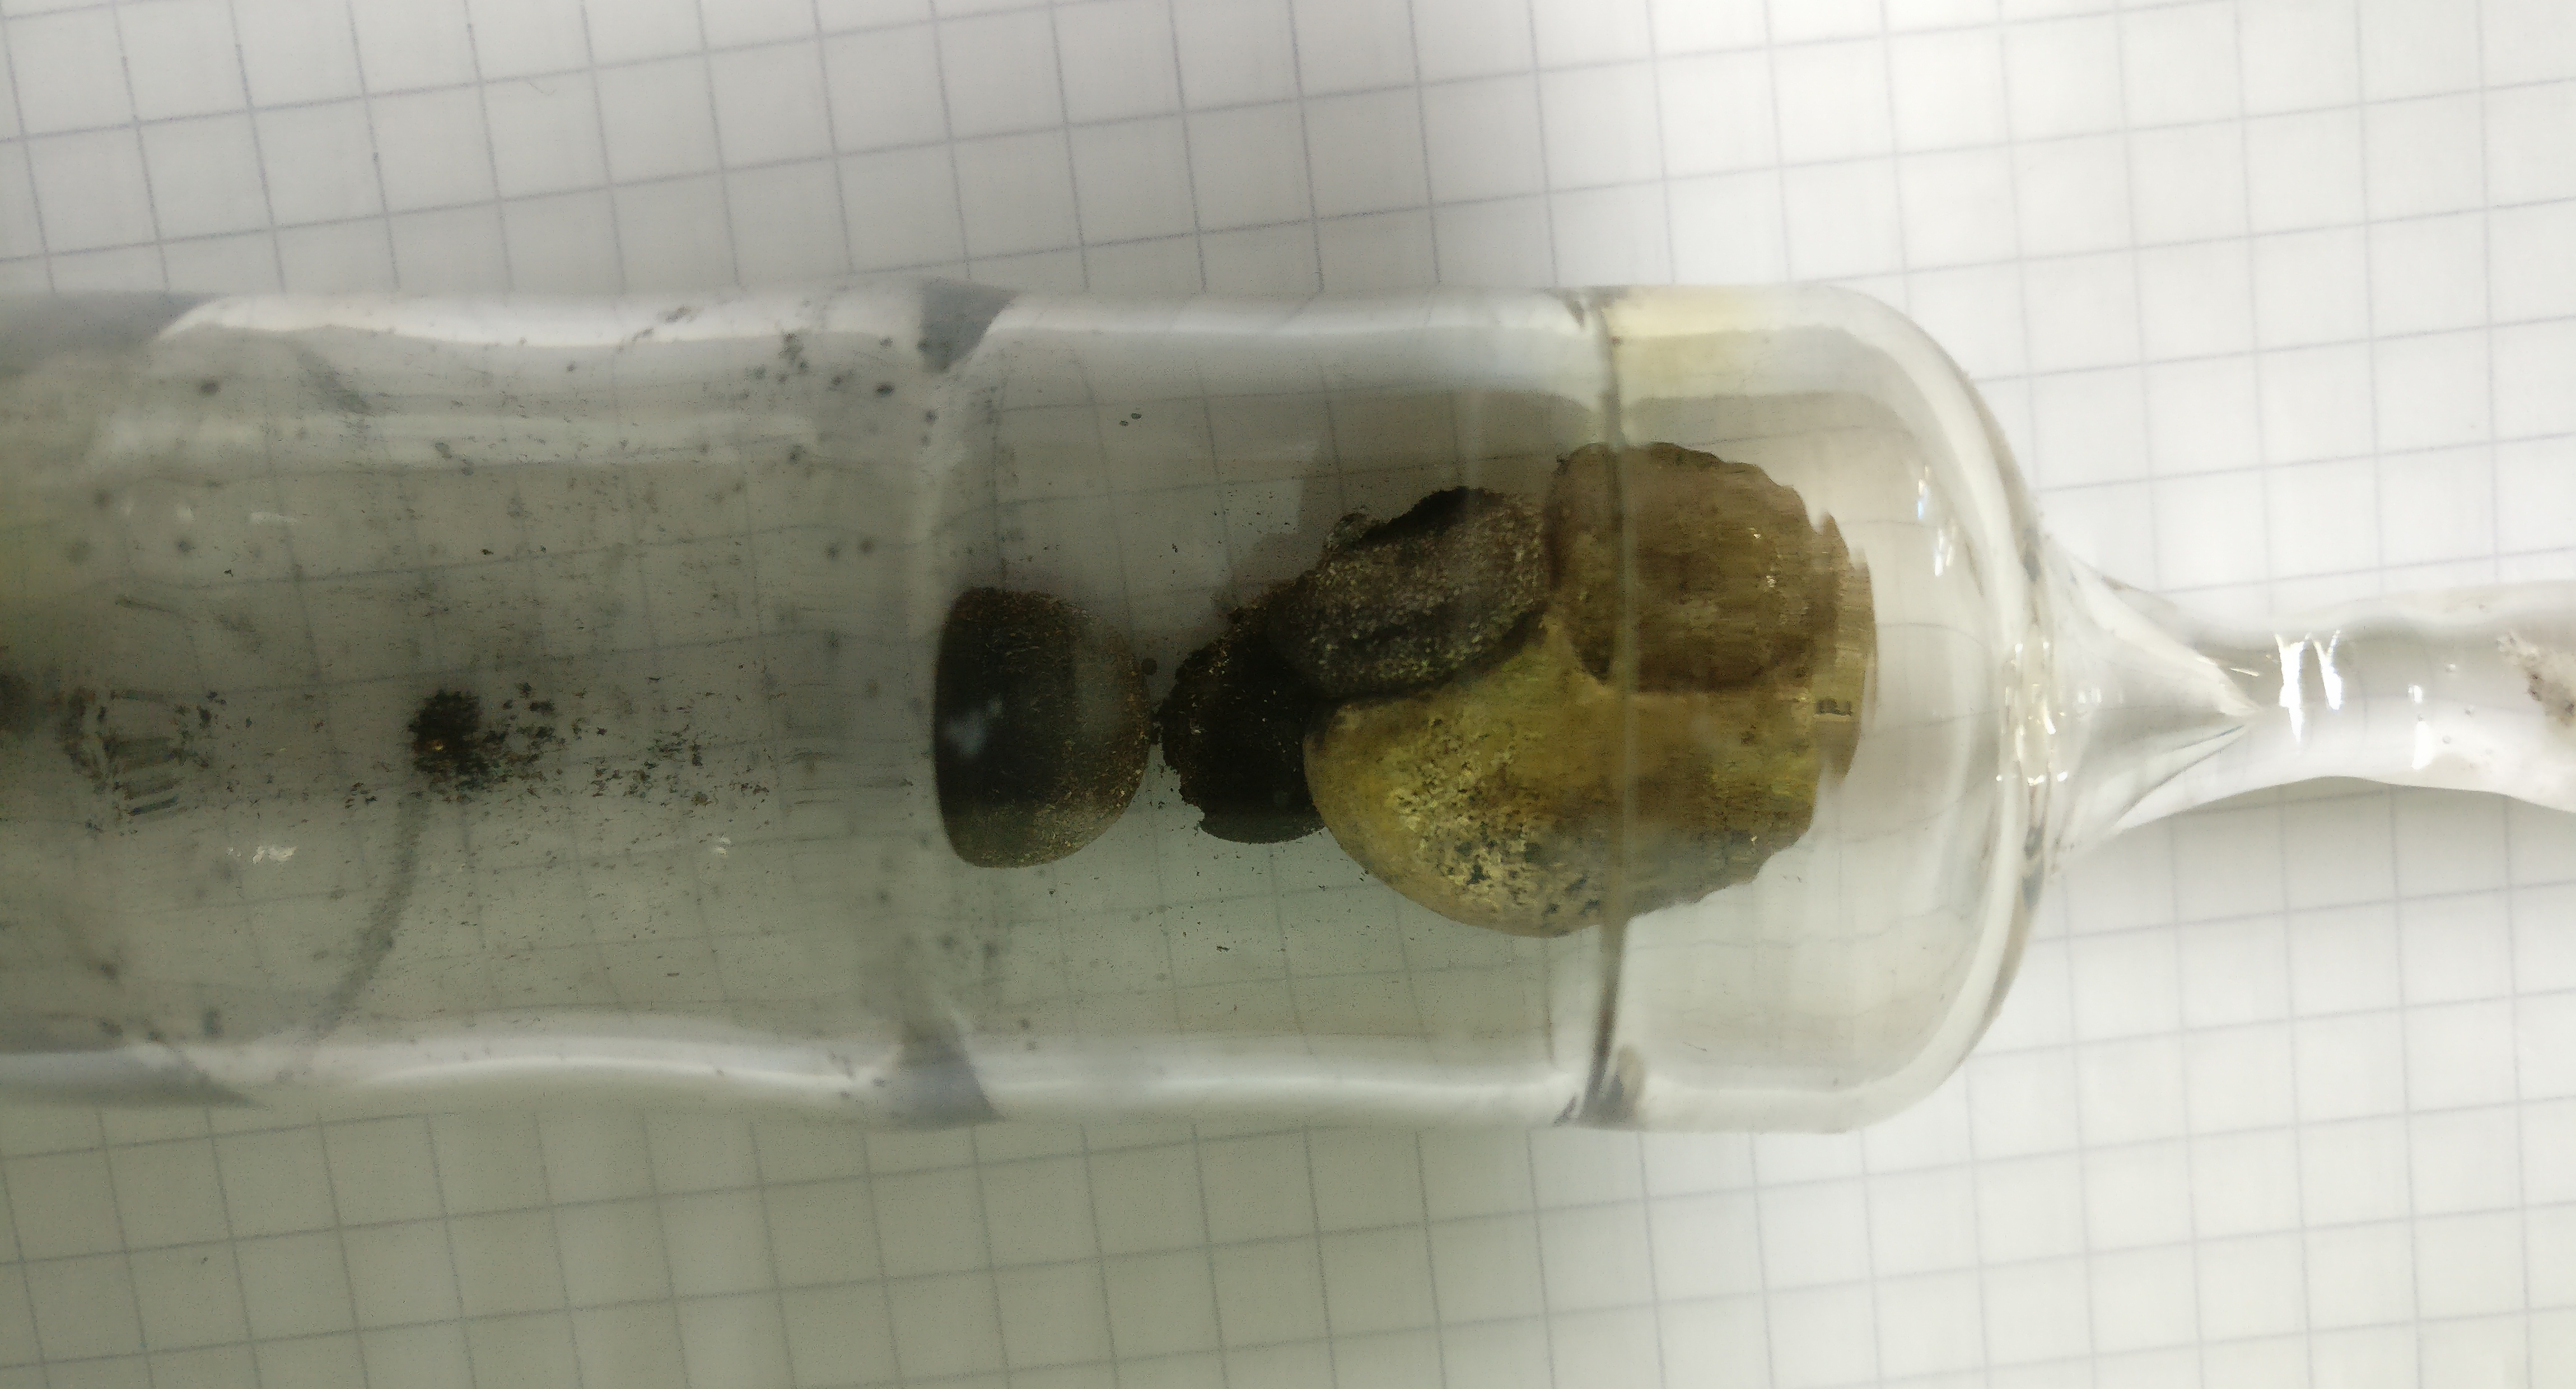
\includegraphics[width=0.32\textwidth]{img/tamgrano/Esponjaypastillas.jpg}


 \end{frame}
%%%%%%%%%%%%%%%%%%%%%%%%%%%%%%%%%%%%%%%%%%%%%%%%%%%%%%%%%%%%%%%%%%%%%%%%%%
% 
% \begin{frame}
%  \begin{center}
% 
% botón y pastillas
%   \end{center}
% \end{frame}







%%%%%%%%%%%%%%%%%%%%%%%%%%%%%%%%%%%%%%%%%%%%%%%%%%%%%%%%%%%%%%%%%%%%%%%%%%%
\begin{frame}

\begin{multicols}{2}

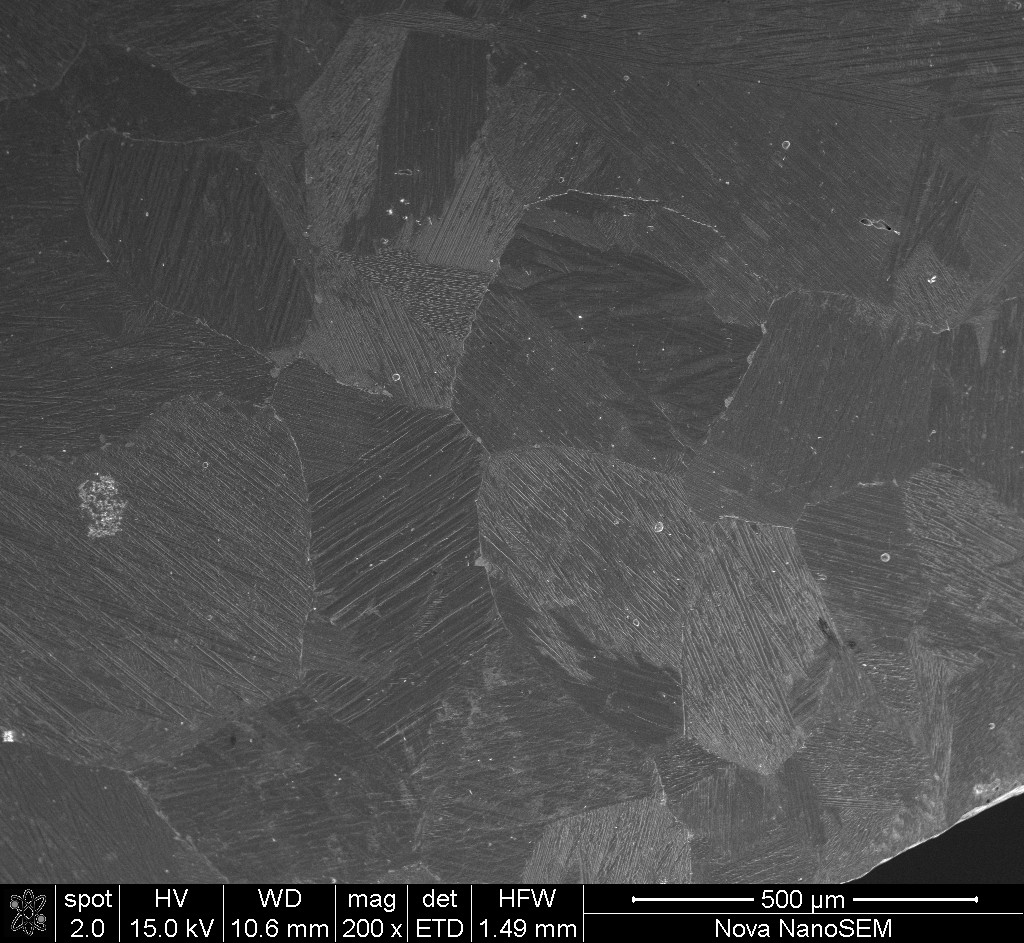
\includegraphics[width=0.5\textwidth]{img/tamgrano/L1B1_016.jpg}

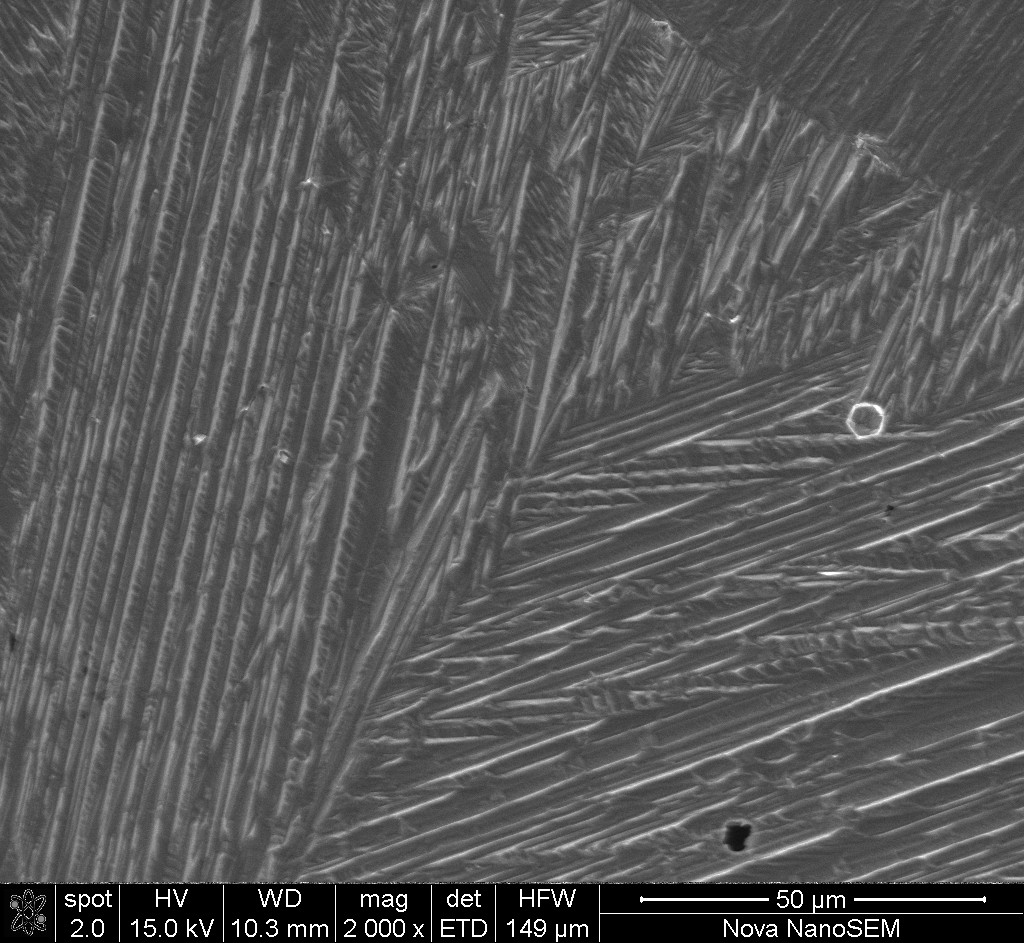
\includegraphics[width=0.5\textwidth]{img/tamgrano/L1B1_014.jpg}
 
\end{multicols}
\end{frame}

% ******************

\begin{frame}
 \frametitle{Disminución tamaño de grano}
\begin{center}
\begin{table} %\label{tab:mstab}
\small
\begin{center}
\begin{tabular}{@{}lllllll@{}}  \toprule
Muestra            & $Cu-Zn-Al (g)$ &   $\% pp$ $AlB_2$ & Método & Horno \\ \midrule
% \alert<1>{Botón 1} & 18,866         & 0,005             & I      & Inducción\\
% \alert<2>{Botón 2} & 18,564         & 0,5               & I      &Resistivo\\
% \alert<3>{Botón 3} & 14,129         & 0,5               & II     &Resistivo \\
% \alert<4>{Botón 4} & 18,383         & 0,5               & II     & Resistivo \\
\alert<1>{Clavo 1} & 8               & 0,5               & III    & Resistivo \\
\alert<2>{Clavo 2} & 8               & 0,05              &III     & Resistivo \\
\alert<3>{Clavo 3} & 8               & -                 & IV   & Resistivo \\
\alert<4>{Clavo 4} & 8               & 0,005             &IV      & Resistivo \\
\bottomrule
\end{tabular}
%\caption{En esta tabla se detallan las composiciones utilizadas en cada muestra, el método de fabricación, y el horno utilizado para la fundición. La composición de la aleación corresponde a aproximadamente $60.115$ $g$ de cobre, $13.714$ $g$ de zinc y $6.130$ $g$ de aluminio. }
\end{center}
\end{table}



\begin{itemize}
\alert<1,2>{\item[Método III:] Aleación $+$ $AlB_2$ papel aluminio $+$ $Cu$} 
\alert<3,4>{\item[Método IV:] Aleación $+$ $AlB_2$ $\rightarrow$  prensado de pastillas}
\end{itemize}
\end{center}


\begin{multicols}{2}

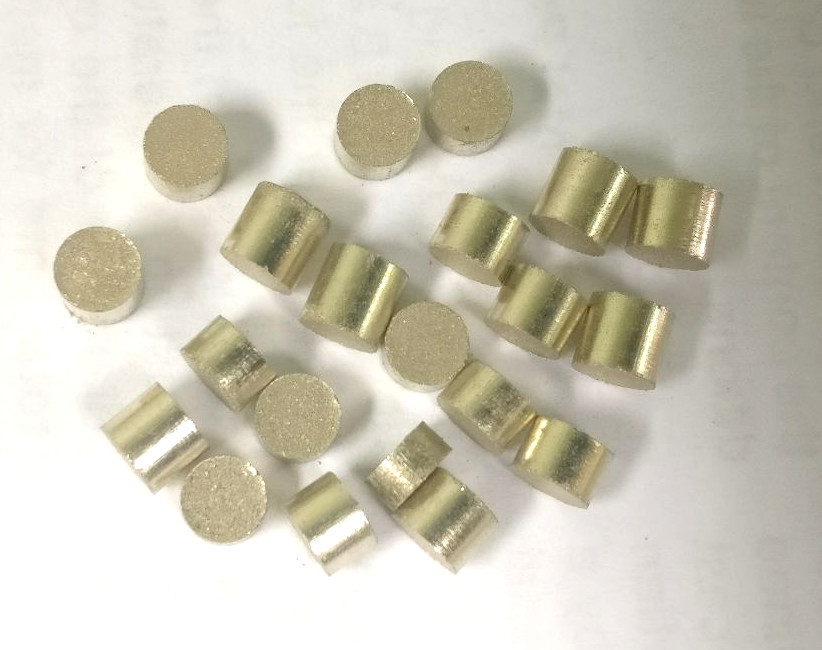
\includegraphics[width=0.2\textwidth]{img/proceso/PastMolienda.jpg}

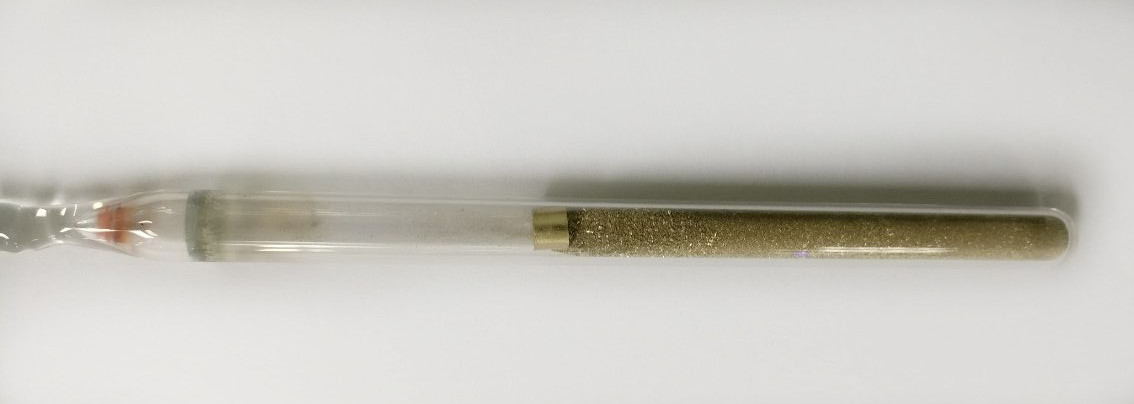
\includegraphics[width=0.4\textwidth]{img/proceso/ClavoPolvo.jpg}

\end{multicols}
 
 \end{frame}
%%%%%%%%%%%%%%%%%%%%%%%%%%%%%%%%%%%%%%%%%%%%%%%%%%%%%%%%%%%%%%%%%%%%%%%%%%%%%%%%%%





\begin{frame}
\begin{center}
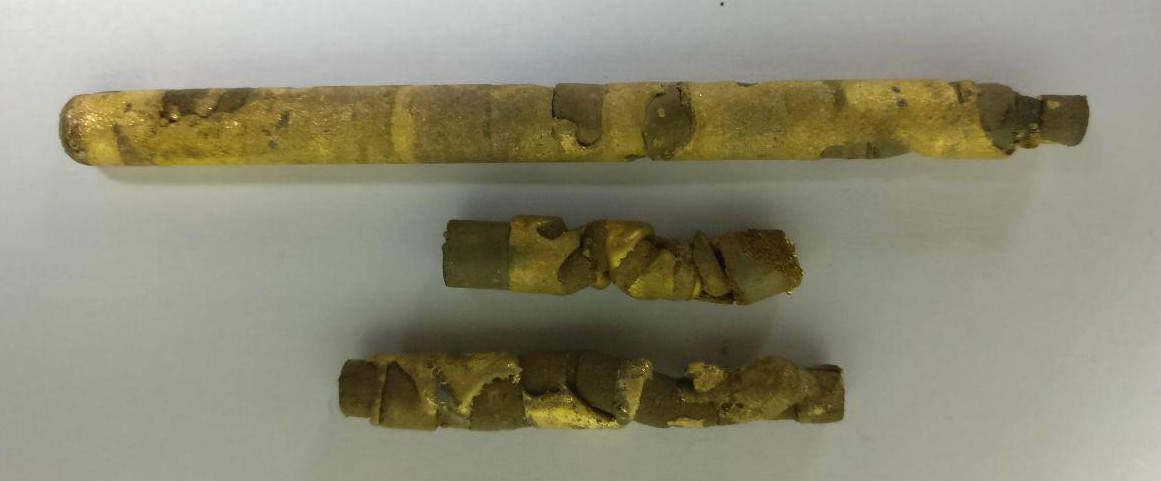
\includegraphics[width=0.60\textwidth]{img/tamgrano/Clavo1_Foto2.jpg} 
\end{center}



 \begin{multicols}{3}
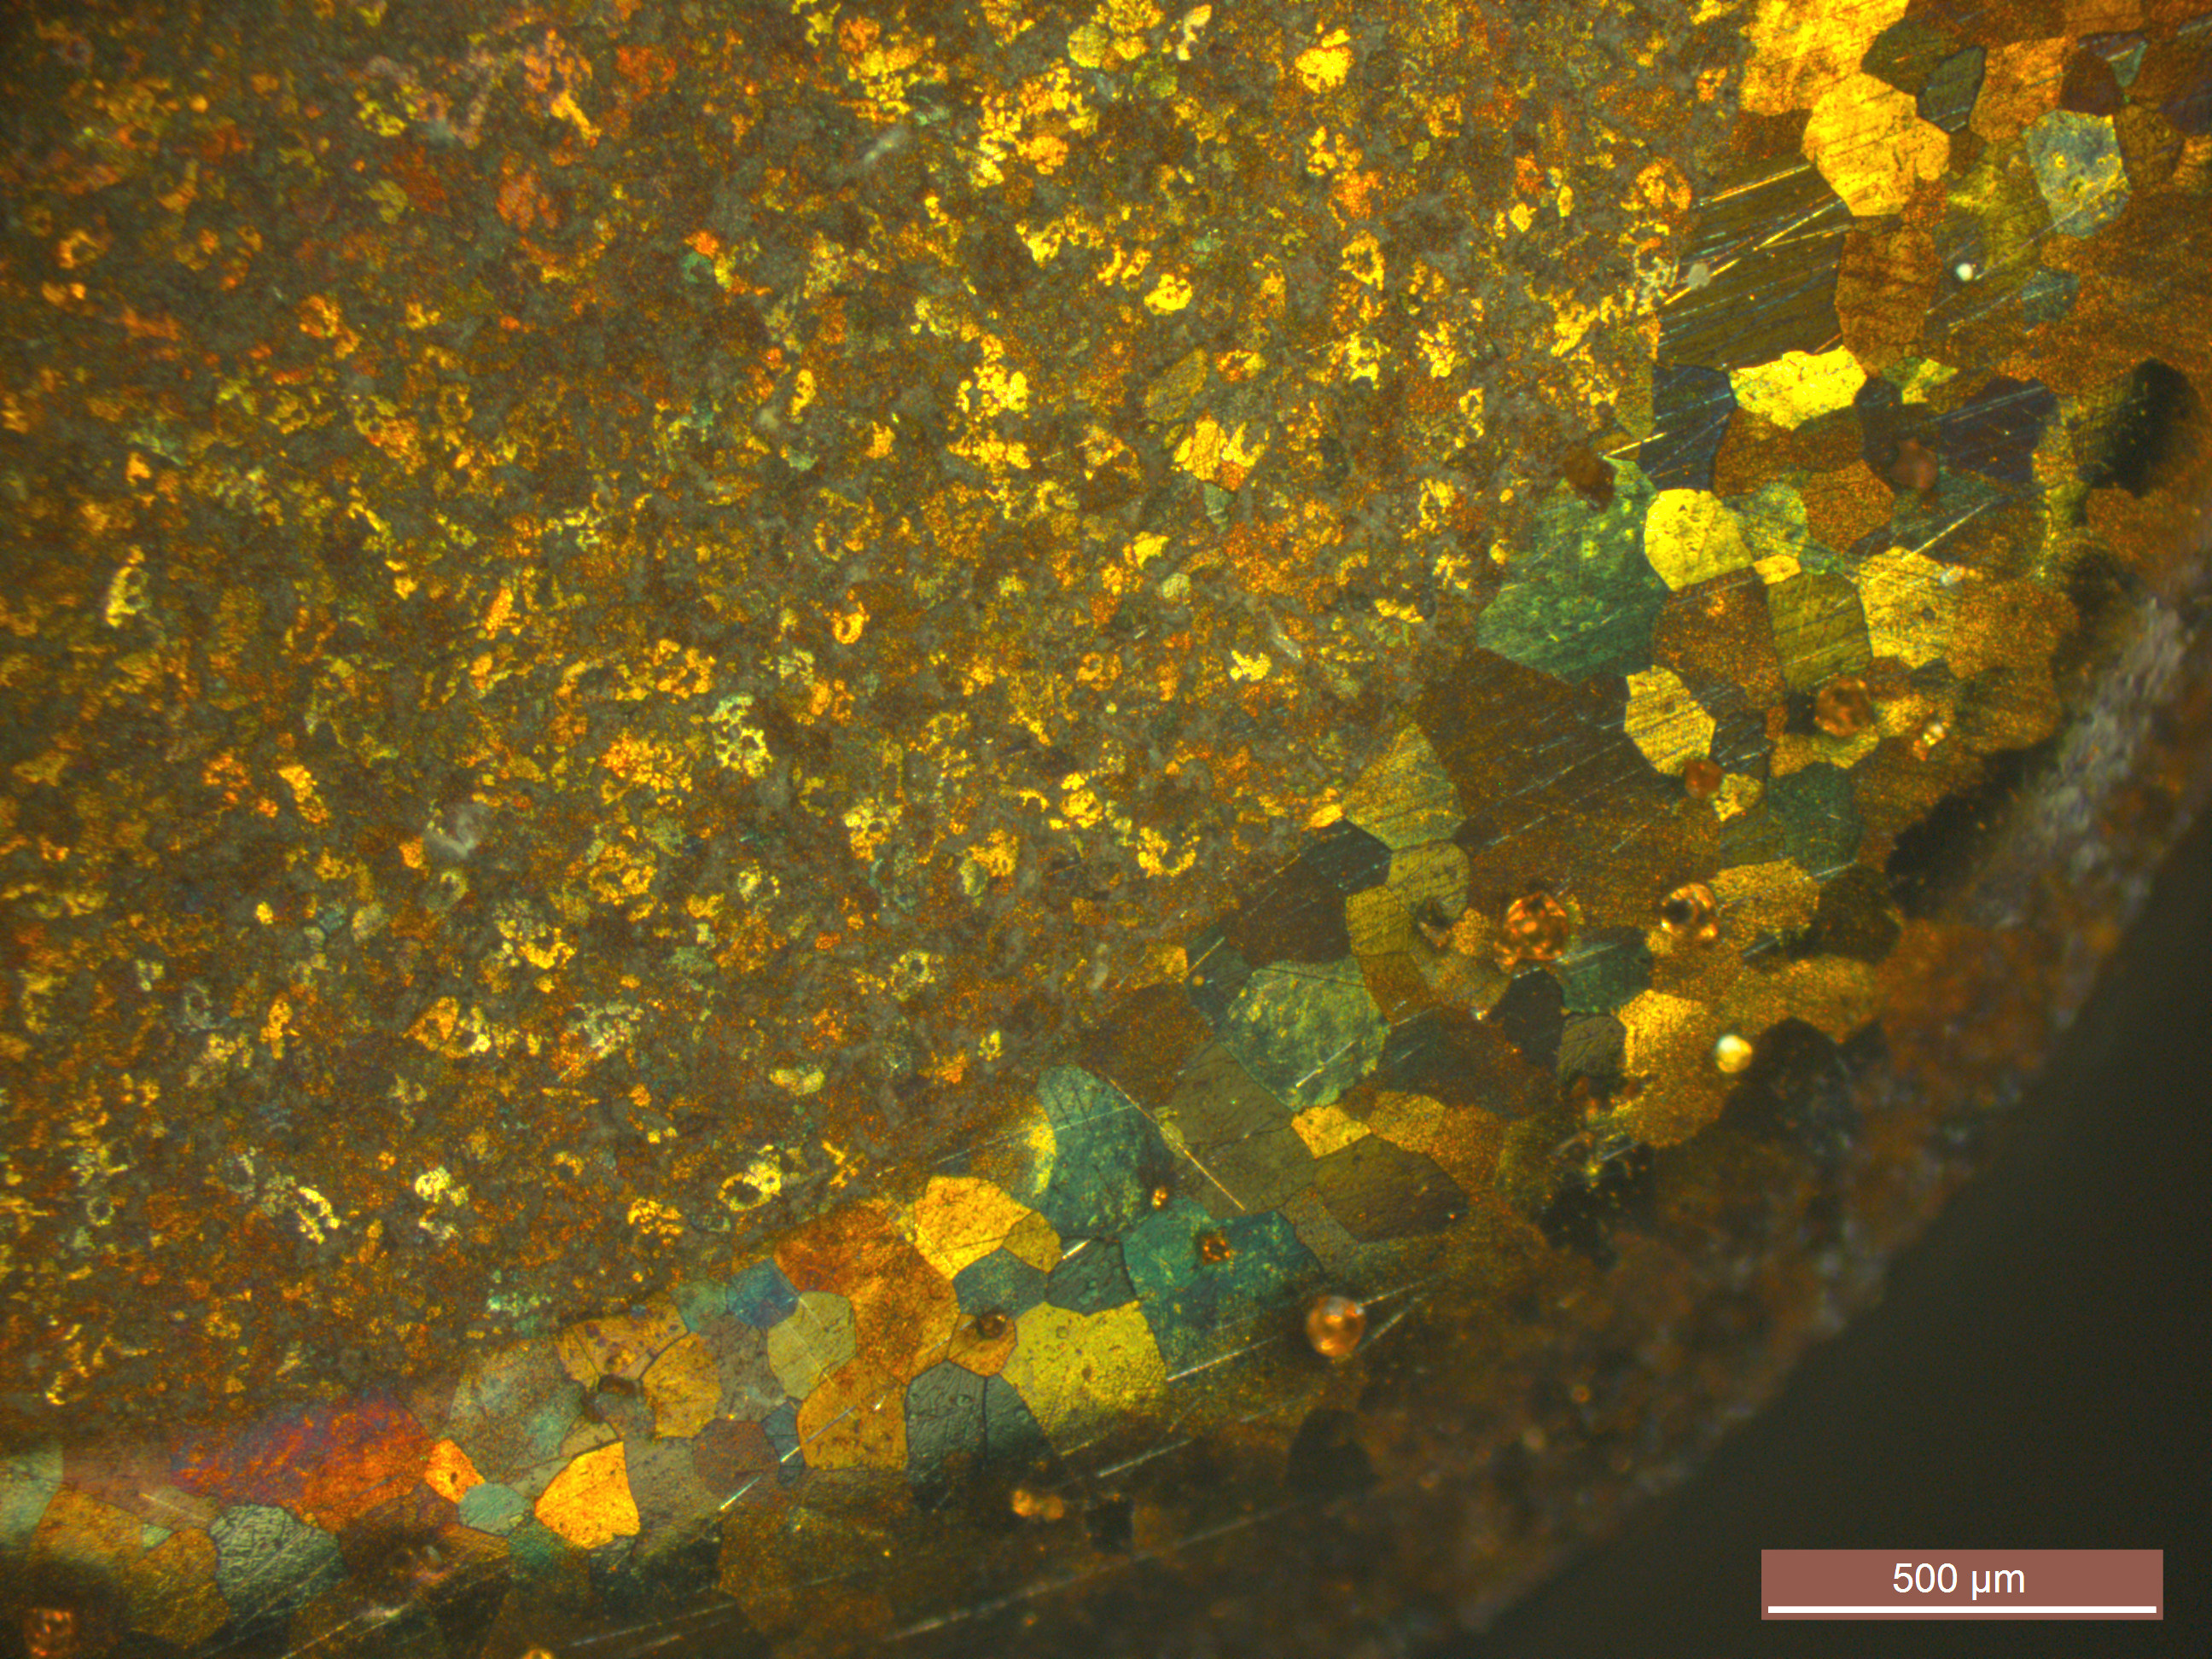
\includegraphics[width=0.37\textwidth]{img/tamgrano/Clavo1.jpg}
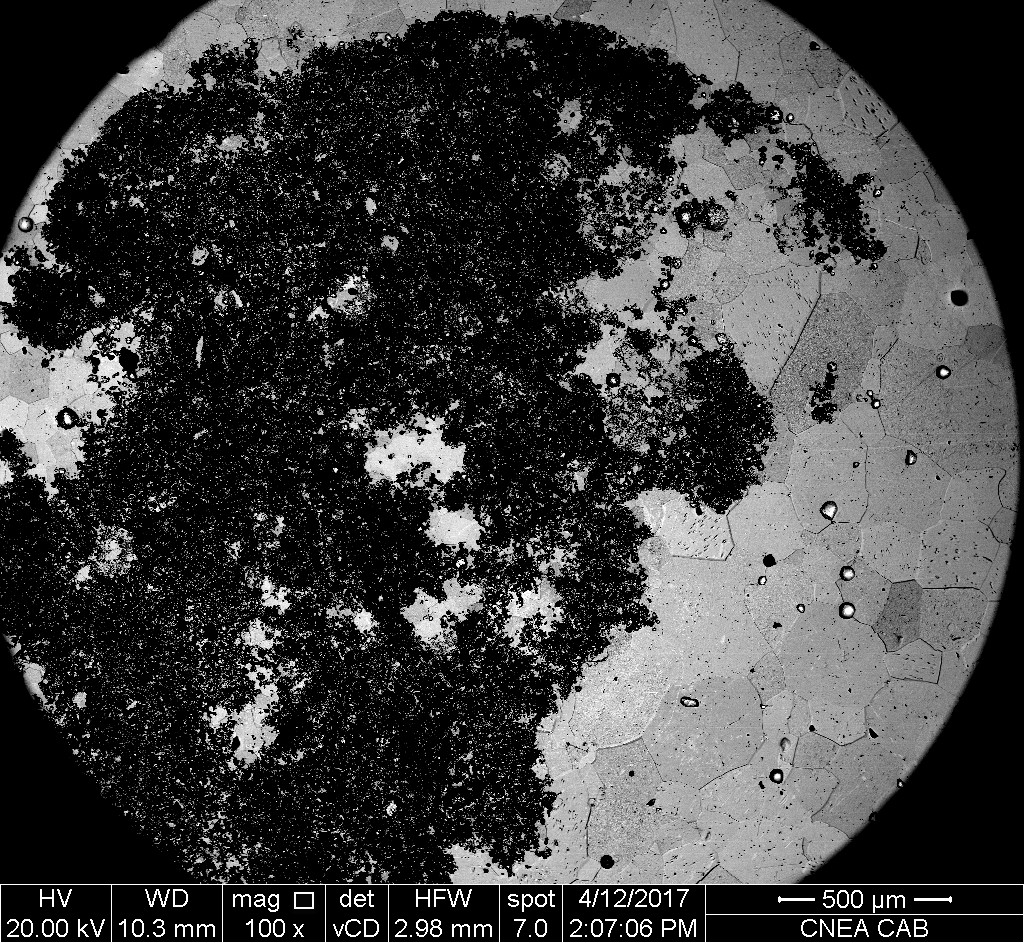
\includegraphics[width=0.3\textwidth]{img/tamgrano/Clavo1Retro.jpg}
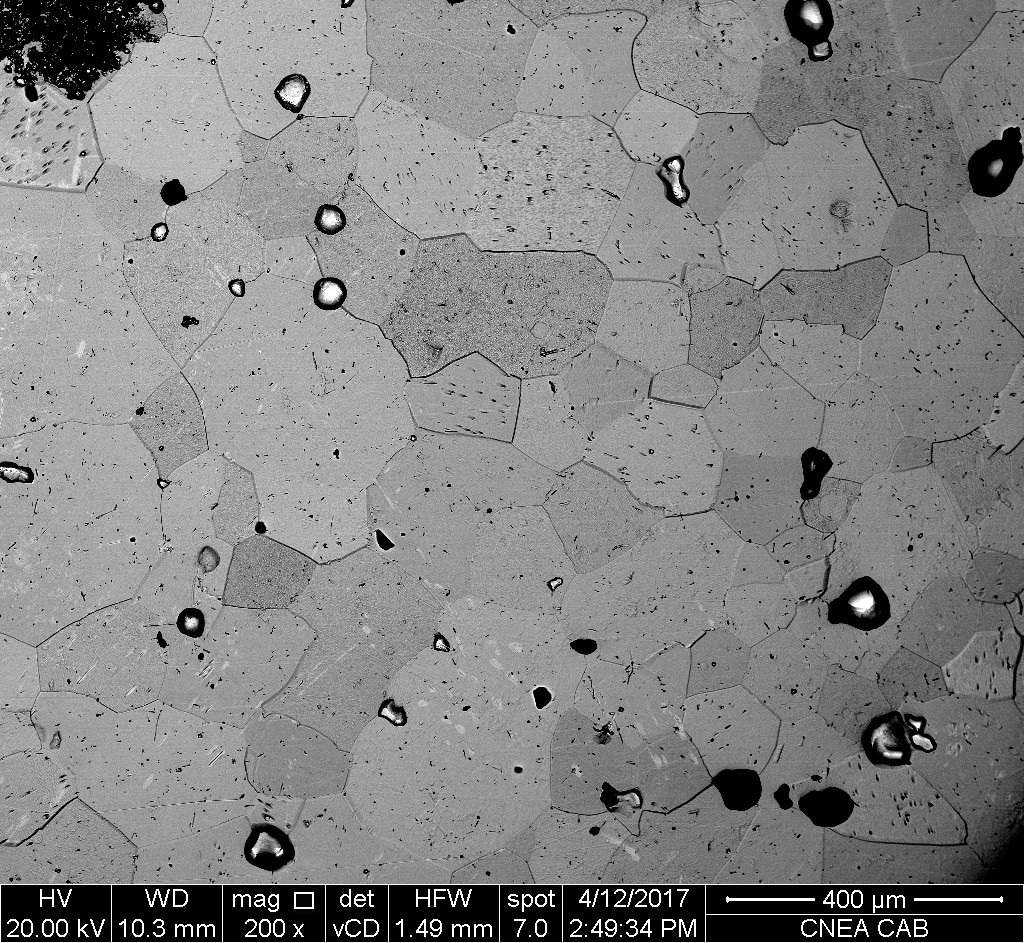
\includegraphics[width=0.3\textwidth]{img/tamgrano/Clavo1Retro2.jpg}
\end{multicols}
\end{frame}





%%%%%%%%%%%%%%%%%%%%%%%%%%%%%%%%%%%%%%%%%%%%%%%%%%%%%%%%%%%%%%%%%%%%%%%%%%%%%%%%%%%%

\begin{frame}
 
 
 
\begin{table} 
\tiny
\begin{center} 
\begin{tabular}{@{}lllll@{}} \toprule
Muestra & $wt \% AlB_2$ & Método de fabricación & $\bar{tg} (mm)$ & $\sigma$ \\ \midrule
 Clavo 5 &  -     & -   & 0.59  & 0.30   \\
 Botón 1    &  0,005 & I   & 0.31 & 0.22  \\
 Clavo 1 &  0,50   & III & 0.16 & 0.08   \\
 Clavo 2 &  0,05  & III & 0.10 & 0.05   \\
 Clavo 3 &  -     & IV  & 0.11 & 0.05   \\
 Clavo 4 &  0,005 & IV  & 0.07 & 0.03   \\
\bottomrule
\end{tabular}
% \caption{Porcentaje de polvo refinador, método de fabricación, valor medio del tamaño de grano ($\bar{tg}$) y desviación media de las distribuciones ($\sigma$) de las distintas muestras fabricadas.}
\end{center}
\end{table}
\begin{center}
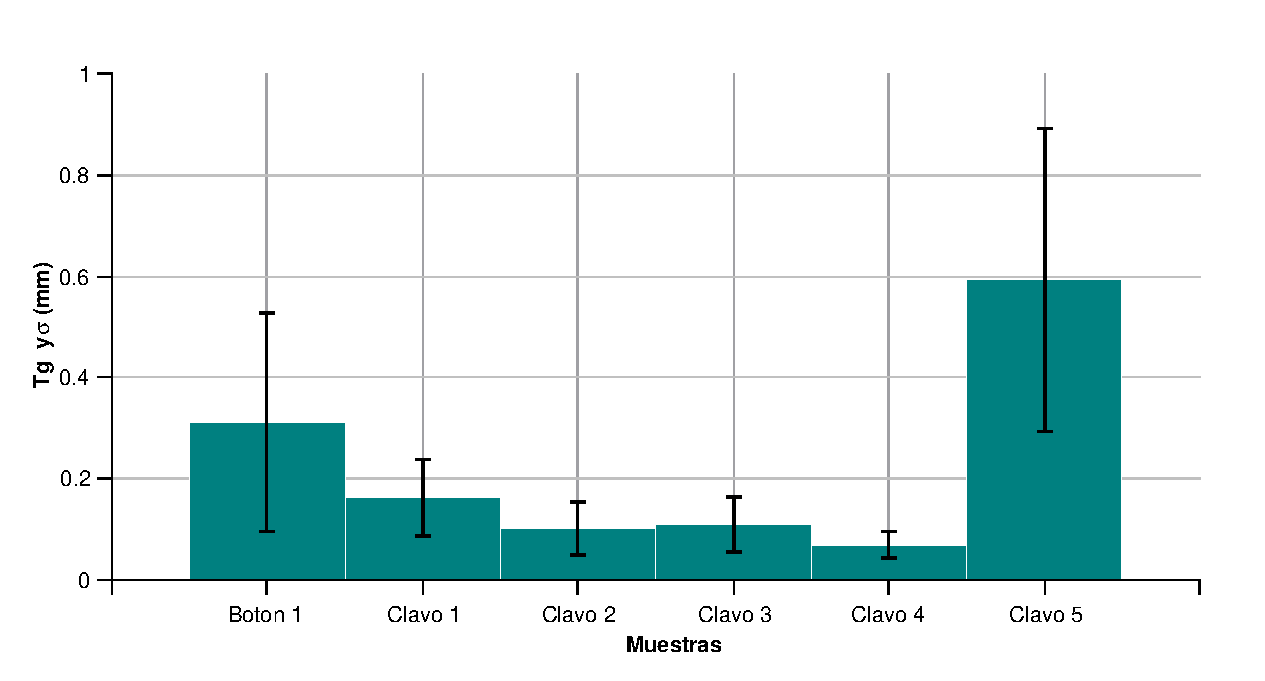
\includegraphics[width=0.7\textwidth]{img/tamgrano/TamGranos.eps}
\end{center}

\end{frame}
%%%%%%%%%%%%%%%%%%%%%%%%%%%%%%%%%%%%%%%%%%%%%%%%%%%%%%%%%%%%%%%%%%%%%%%%%%%%%%%%%%%%%%%%%%%%%%%%%%%%%%%%%%%%%%%%%

\begin{frame}
 \begin{center}
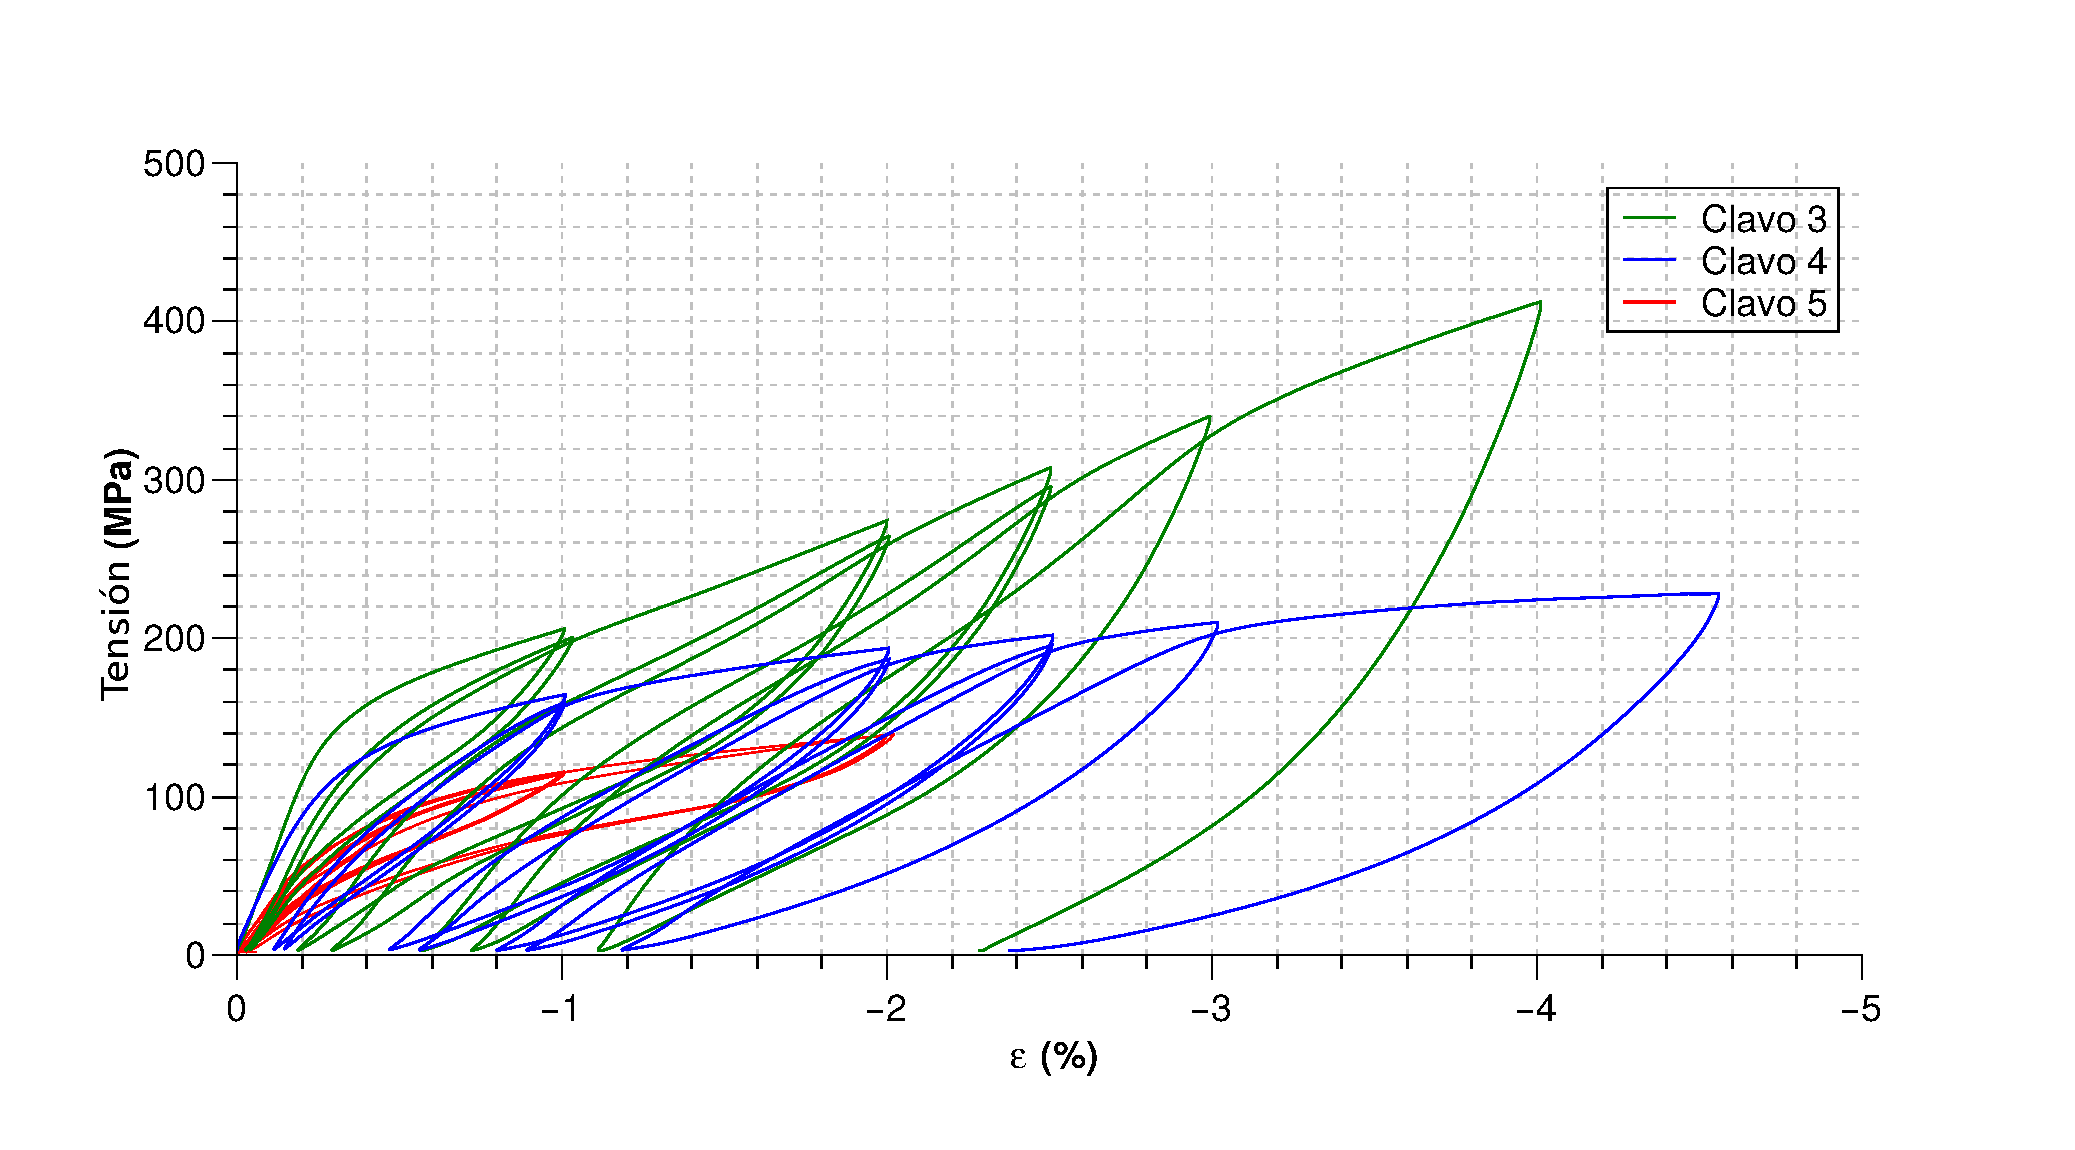
\includegraphics[width=0.9\textwidth]{img/tamgrano/Clavos_3_4_5.eps}
\end{center}

\end{frame}



%%%%%%%%%%%%%%%%%%%%%%%%%%%%%%%%%%%%%%%%%%%%%%%%%%%%%%%%%%%%%%%%%%%%%%%%%%%%%%%%%%%%%
\begin{frame}

%\begin{multicols}{2}
\begin{center}

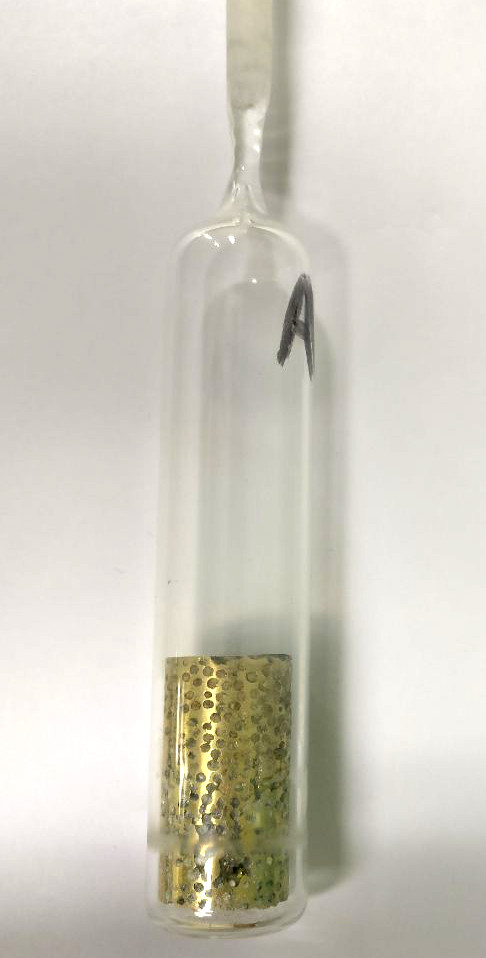
\includegraphics[width=0.2\textwidth]{img/tamgrano/EspCuarzo.jpg}
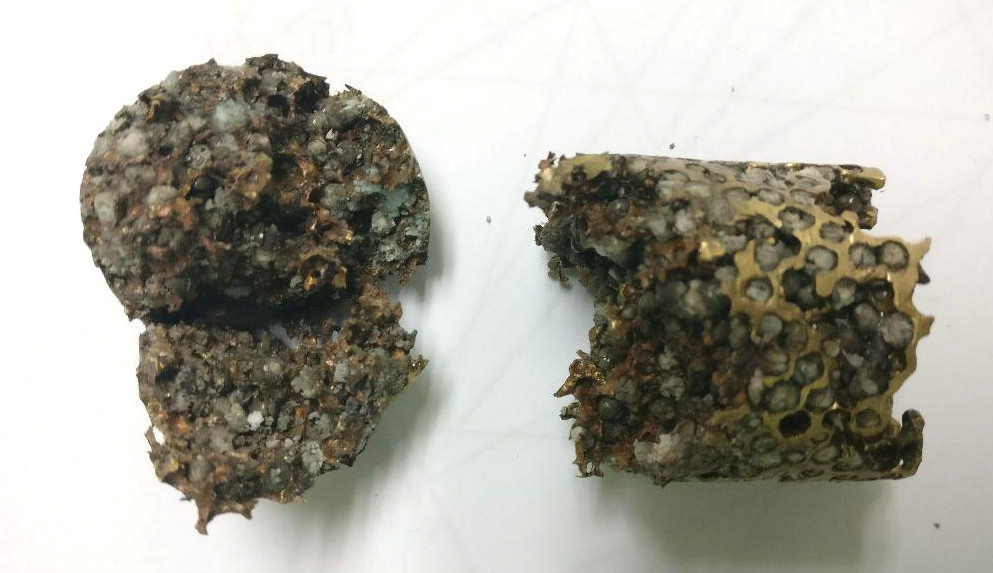
\includegraphics[width=0.6\textwidth]{img/tamgrano/EspRota.jpg}

\end{center}
%\end{multicols}



\end{frame}

%***************************

\subsection{Resistencia}

% ******************
\begin{frame}
 Introducción
 
  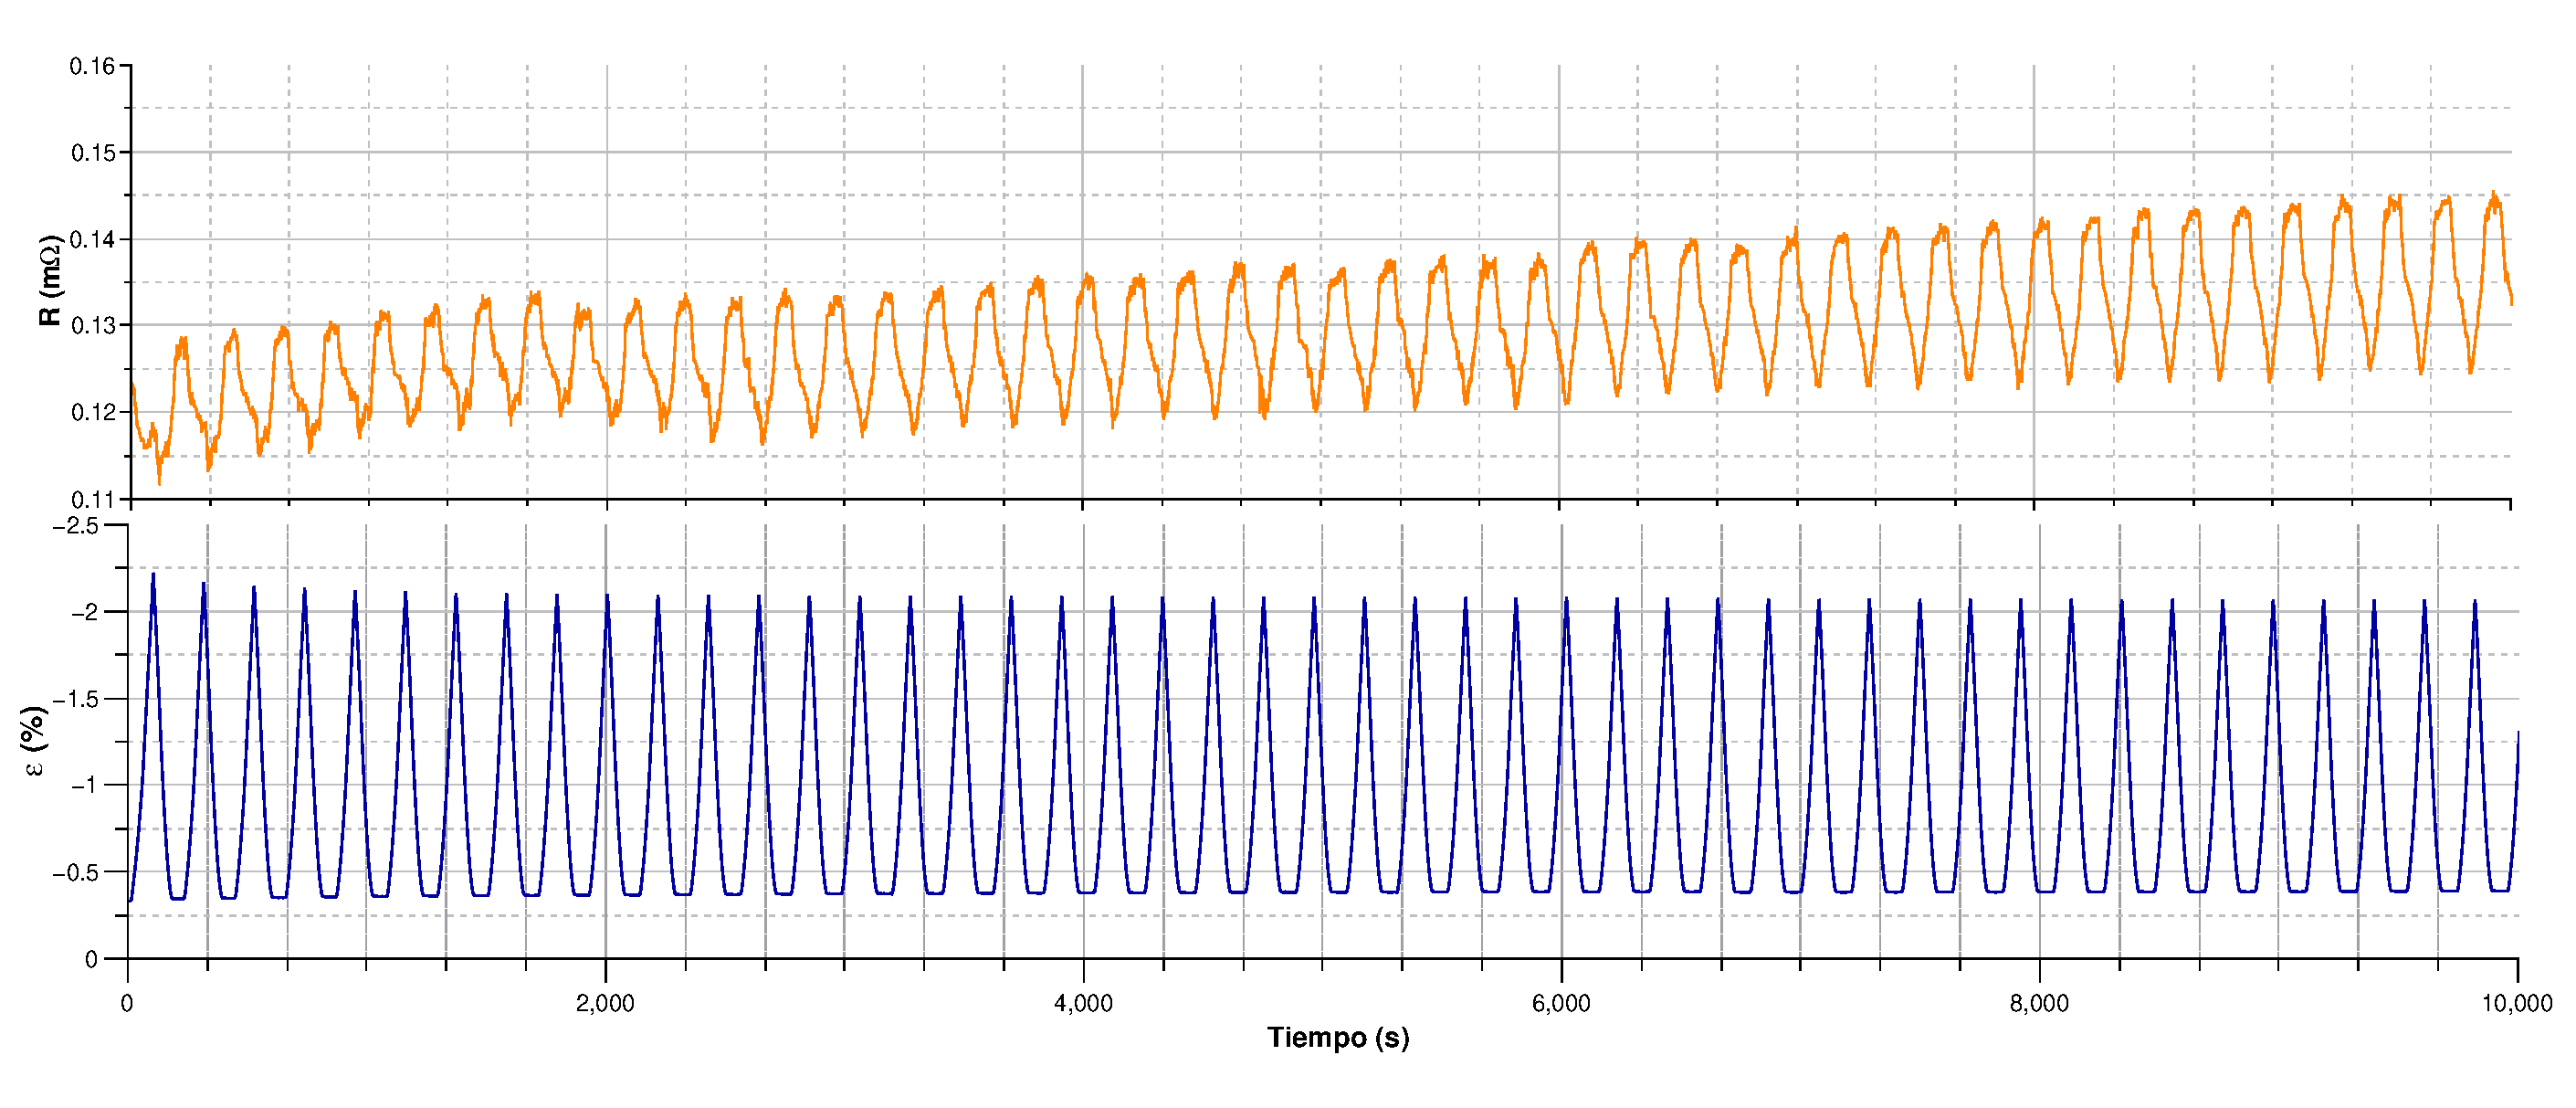
\includegraphics[width=0.95\textwidth]{img/resistencia/Ciclos.eps}

\end{frame}

% ******************

\begin{frame}
\frametitle{Metodo cuatro puntas}

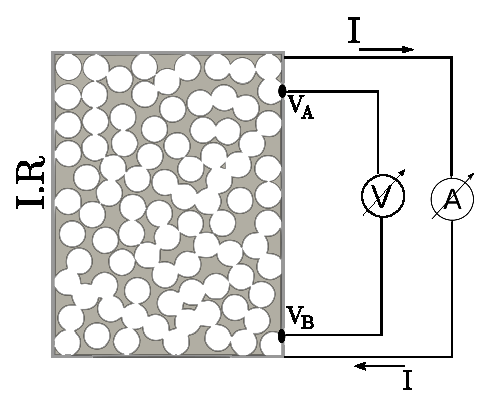
\includegraphics[width=0.4\textwidth]{img/resistencia/CuatroPuntas1.eps}
\includegraphics[width=0.4\textwidth]{img/resistencia/cpfoto.png}

\begin{equation*}
V^+= V_A +I^+ . R - V_B 
\end{equation*}
\begin{equation*}
 V^-= V_A +I^- . R - V_B 
\end{equation*}
\begin{equation*}
 V^+ - V^-= [I^+ + I^-] R \longrightarrow R=\frac{V^+ - V^-}{(I^+ + I^-)}
\end{equation*}
\begin{equation*}
 \rho = R . \frac{A}{l} \label{resist} 
\end{equation*}


\end{frame}

%%%%%%%%%%%%%%%%%%%%%%%%%%%%%%%%%%%%%%%%%%%%%%%%%%%%%%%%%%%%%%%%%%%%%
\begin{frame}
        \includegraphics[width=0.4\textwidth]{img/resistencia/EjTensionDef.eps}
%        \includegraphics[width=\textwidth]{Img/resistencia/Ejblanco.jpg}
        \includegraphics[width=0.4\textwidth]{img/resistencia/EjTempDef.eps}
\newline
        \includegraphics[width=0.4\textwidth]{img/resistencia/EjTempRes.eps}

Descripción histéresis 

\end{frame}
%%%%%%%%%%%%%%%%%%%%%%%%%%%%%%%%%%%%%%%%%%%%%%%%%%%%%%%%%%%%%%%%%%%%5


\begin{frame}
 \begin{equation}
 R_0= \rho \frac{l_0}{A_0}
\end{equation}
donde $R_0$ ($\Omega$) es la resistencia inicial, $\rho$ ($\Omega m$) es la resistividad, $l_0$ es el largo inicial y $A_0$ la sección inicial. 
%
\begin{equation*}
 l=l_0 * (1+ \varepsilon)
  \quad \quad y \quad \quad  
 A=\frac{A_0}{(1+ \varepsilon)} \quad 
\end{equation*}
Por lo tanto, 
\begin{equation}
R= \rho \frac{l}{A} = \rho (1+\varepsilon)^2 \frac{l_0}{A_0} = (1+\varepsilon)^2 R_0 %= \rho f^2 \frac{l_0}{A_0}
\end{equation}

De esta manera, $(1+\varepsilon)^2$ es un factor que relaciona el cambio de la resistencia con los cambios geométricos de la muestra. 
\end{frame}




% ******************

\begin{frame}
\begin{equation*}
  \rho_M =f \rho_A
\end{equation*}
\begin{equation*}
 R_M^0 =fR_A   
 % \longrightarrow    \rho_M=f\rho_A 
\end{equation*}

En este caso se está tomando en cuenta la compresión que sufre la muestra al transformar, que generará una disminución en la resistencia, y entonces llegará al valor ${R_M}$. Por lo tanto tendremos:
\begin{equation*}
 {R_M}=f'R_A 
\end{equation*}
donde $f'$ es el factor que relaciona las resistencias en un experimento real. Como $R_M=R_M^0 (1+\varepsilon)^2 = f' R_A$ se llega a:
\begin{equation*}
 R_M^0 (1+\varepsilon)^2 = f'R_A
\end{equation*}
\begin{equation*}
f' = f (1+\varepsilon)^2  \label{fprima}
\end{equation*}
Esta ecuación relaciona los valores de resistencia al transformar, tomando en cuenta los cambios geométricos en la muestra. 

\end{frame}

% ******************

%%%%%%%%%%%%%%%%%%%%%%%%%%%%%%%%%%%%%%%%%%%%%%%%%%%%%%%%%%%%%%%%%%%%%%%%%%%%%%%%%%%%%%%%%%%%%%%%%%%%%%%%%%%%%%%

\begin{frame}
        \includegraphics[width=0.5\textwidth]{img/resistencia/ExpRes.eps}
        \includegraphics[width=0.7\textwidth]{img/resistencia/ExpStrain.eps}
\end{frame}

%%%%%%%%%%%%%%%%%%%%%%%%%%%%%%%%%%%%%%%%%%%%%%%%%%%%%%%%%%%%%%%%%%%%%%%%%%%%%%%%%%%%%%%%%%%%%%%%%%%%%%%%%%%%%%%%%

\begin{frame}
 
 \begin{figure}
 \includegraphics[width=0.6\textwidth]{img/resistencia/PoliMono2.eps}
% \caption{Gráficos obtenidos al realizar ciclos de compresión de una esponja de Cu-Zn-Al hasta $-2\%$ de deformación. Abajo se muestra un gráfico de la deformación en función del tiempo y arriba los correspondientes valores de resistencia. } 
 \end{figure}

 \begin{multicols}{2}
 
\begin{table} 
\tiny
\begin{tabular}{@{}llllll@{}} \toprule
Tensión ($MPa$) & $\varepsilon$ ($\%$) &  $f'=\frac{R_M}{R_A}$\\ \midrule
 0        &  0.76   & 1.27\\
 1.93       &  0.37   & 1.28\\
 17.4      &  -7.60  & 1.15\\
 31.0      &  -7.90  & 1.17\\
 46.5     &  -8.00  & 1.17  \\
 Referencia    & 8.00  &  1.73   \\
 \bottomrule
\end{tabular}
 \caption{Monocristal}
%Resultados obtenidos al realizar ciclos térmicos de transformación con distintas cargas aplicadas con un monocristal de Cu-Zn-Al. En la primera columna se muestran las cargas aplicadas que se mantuvieron constantes durante cada ciclo de transformación, $\varepsilon$ es la deformación máxima registrada por el extensómetro al transformar completamente a martensita, $f=\frac{R_M}{R_A}$ es el cociente entre la resistencia en estado martensítico y el estado austenítico.}
\end{table}

 
\begin{table}
\tiny
\begin{center} 
\begin{tabular}{@{}llllll@{}} \toprule
Tensión (Mpa) & $\varepsilon$ ($\%$) &  $f'=\frac{R_M}{R_A}$\\ \midrule
 0        &  -0.10   & 1.30\\
 0       &  -0.60   & 1.27 \\
 0      &  -0.50   & 1.28 \\
 2.04      &  -0.90  & 1.27\\
 18.4    &  -1.60  & 1.24 \\
32.7      &  -2.60 & 1.21\\
 49.1     &  -2.50  & 1.23   \\
 \bottomrule
\end{tabular}
 \caption{Policristal}
%Resultados obtenidos al realizar ciclos térmicos de transformación con distintas cargas aplicadas con un policristal de Cu-Zn-Al. En la primera columna se muestran las cargas aplicadas que se mantuvieron constantes durante cada ciclo de transformación, $\varepsilon$ es la deformación máxima registrada por el extensómetro al transformar completamente a martensita, $\frac{R_M}{R_A}$ es el cociente entre la resistencia en estado martensítico y el estado austenítico. También se esquematiza que $f$ corresponde a la pendiente de la recta.}
\end{center}
\end{table}
 
\end{multicols}
 
 
\end{frame}

% ******************

\begin{frame}

\includegraphics[width=0.7\textwidth]{img/resistencia/Histeresis2.eps}

\end{frame}

% ******************
\begin{frame}
 Al concluir un ciclo de transformación a martensita y volver a austenita, la resistencia estará dada por:
\begin{equation}
 R^A _i=\rho^A \frac{L_0}{A_i}(1-b_i) + \rho^M \frac{L_0}{A_i}b_i = \rho^A \frac{L_0}{A_i} [1+ b_i (f-1)]
\end{equation}
Donde ahora $0<b_i <1$ representa la fracción de martensita retenida luego de ese ciclo de transformación y $(1-b_ i)$ la aleación restante que transforma a austenita. En este punto, la resistencia estará dada por la austenita, martensita retenida, y además por la rotura de la estructura. Por ejemplo luego del primer ciclo de transformación será $R^A _{1}$ en la figura. 
Si en el estado inicial la esponja esta compuesta solo por austenita y no presenta ninguna rotura su resistencia estará dada por:
\begin{equation}
 R^A _0 = \rho^A \frac{L_0}{A_0}
\end{equation}
\end{frame}


\begin{frame}
Por lo tanto en el ciclo $i$ de transformación la resistencia en estado austenítico será:
\begin{equation}
 R^A _i = R^A _0 \frac{A_0}{A_i} [1+b_i (f-1)]=R^A _0 a_i [1+b_i (f-1)] \label{austenita}
\end{equation}

Si ahora comparamos le resistencia inicial en estado austenítico $R^A _0$ con la resistencia en estado martensítico luego del ciclo $i$ de transformación obtendremos:

\begin{equation}
 R^M _i = \rho ^M \frac{L_0}{A_i}
\end{equation}
Si el parámetro $f$ relaciona las resistividades en estado austenítico y martensítico, entonces:
\begin{equation}
 f=\rho^M / \rho^A \longrightarrow
 R^M _i = f R^A _0 \frac{A_0}{A_i} = R^A _0 a_i f \label{martensita}
\end{equation}

\end{frame}

% ******************

\begin{frame}

\begin{multicols}{2}
  \begin{table} 
 \tiny
 \begin{center} 
  \begin{tabular}{@{}lllllll@{}} \toprule
  Esponja & Ensayo   &    $R^M$    &  $R^A$ &  $A_0/A$ \\ \midrule
  1   & 1       &  0.040  & 0.031 & 1.009  \\
  1   & 2       &  0.046  & 0.034 &  1.061  \\
  1   & 3       &  0.058  & 0.042 &  1.067  \\
  1   & 4     &  0.089  & 0.068 &  1.010 \\
  2   & 1     &  0.015  & 0.011 &  0.992  \\
  2   & 2    &  0.017  & 0.013 &  1.007   \\
  \bottomrule
% ************************************************   GRAFICOS ESPONJA D
  \end{tabular}
%\caption{Parámetro $A/A_0$ calculado para las esponjas de Cu-Zn-Al en distintos ensayos a partir de los datos obtenidos del gráfico. Se ve como con cada ensayo el área de la esponja disminuye respecto del área inicial.}
%\label{tab:A0Arotura}
\end{center}
  \end{table}


% ******************


\begin{table} 
\tiny
\begin{center} 
\begin{tabular}{@{}lllllll@{}} \toprule
Esponja &Ensayo   &    $R^M$    &  ${R^A}$ &  b \\ \midrule
1 & 1       &  0.031  & 0.031   & 0.033  \\
1 & 2       &  0.035  & 0.034  &  0.139  \\
1 & 3       &  0.044  & 0.042  &  0.166  \\
1 & 4      &  0.069 &	0.068 &	0.044 \\
2 & 1      &  0.011 &	0.011 & 0.029 \\
2 & 2      &  0.013 &	0.012 & 0.054\\
 \bottomrule

 \end{tabular}
%\caption{Valores de martensita retenida ($b$) obtenidos para las esponjas 1 y 2 de Cu-Zn-Al utilizando los valores del gráfico \ref{fig:RED_resultados} }

\end{center}
\end{table}

\end{multicols}
\end{frame}

% ******************

\begin{frame}
 Conclusiones
\end{frame}


\end{document}